\documentclass[a4paper,11pt]{ltjsarticle}
\usepackage{geometry}
\geometry{top=25mm,bottom=25mm,left=25mm,right=25mm}
\usepackage{graphicx}
\usepackage{amsmath,amssymb,bm}
\usepackage{hyperref}
\usepackage{float}

\hypersetup{
  pdftitle={数理工学実験レポート 第2章(数値線形代数)},
  pdfauthor={中塚 一瑳}
}

\title{数理工学実験レポート\\\vspace{5pt}\large 第2章(数値線形代数)}
\author{学籍番号 1029366161\quad 中塚 一瑳}
\date{\today}

\begin{document}

% 表紙(1ページ)
\begin{titlepage}
\centering
{\Large 数理工学実験レポート\par}
\vspace{4mm}
{\large 第1章(数値線形代数)\par}
\vspace{15mm}
{\large 京都大学 工学部情報学科 数理工学コース\par}
{\large 学年:2回生\par}
{\large 学籍番号:1029366161\quad 中塚 一瑳\par}
\vspace{10mm}
\begin{tabular}{@{}ll}
科目名: & 数理工学実験 \\
実験テーマ: & 数値線形代数 \\
実験の実施年月日: & \today \\
レポート提出年月日: & \today \\
\end{tabular}
\vfill
\end{titlepage}

\section*{要旨(Abstract)}


\section{はじめに}
本章では,数値計算の基礎となる数値線形代数の手法を取り上げる.
連立一次方程式や固有値問題の数値的解法を通じて,計算精度・安定性・効率性の観点から
各アルゴリズムの特徴を理解することを目的とする.
また,理論的背景と実装結果を比較し,数値誤差や収束挙動の要因を考察することで,
線形代数の理論と計算機実装の関係を体系的に把握することを目指す.

% ===== 課題ごとの構成 =====

\section{課題1:ガウスの消去法による連立一次方程式の解法}

\subsection{原理・方法}
ガウスの消去法は,連立一次方程式
\[
A\boldsymbol{x} = \boldsymbol{b}
\]
を上三角化によって逐次的に解く手法である\cite{exp2025}.行基本変形により係数行列 $A$ を上三角行列 $U$ に変換し,対応して右辺 $\boldsymbol{b}$ にも同じ操作を施す.これにより
\[
U\boldsymbol{x} = \boldsymbol{c}
\]
の形が得られ,最後に後退代入(back substitution)を行うことで未知ベクトル $\boldsymbol{x}$ を求める.

各ステップでは,ピボット要素 $A_{k,k}$ を基準に第 $k$ 列の下部要素を消去する.ただし $A_{k,k}$ が小さいと丸め誤差の影響で数値不安定となるため,絶対値が最大の要素を選んで行を入れ替える「主成分選択(partial pivoting)」を導入する.これにより除算時の誤差伝播が抑制され,計算の安定性が向上する.

Julia による実装例を以下に示す.

\begin{verbatim}
function gaussian_elimination(A)
    A = float.(copy(A))            # 浮動小数点型への変換
    n = size(A, 1)
    for k = 1:n-1
        # --- 主成分選択 ---
        pivot = k - 1 + argmax(abs.(A[k:end, k]))
        if pivot != k
            A[k, :], A[pivot, :] = A[pivot, :], A[k, :]
        end

        # --- 消去操作 ---
        for i = k+1:n
            if A[i,k] != 0
                factor = A[i,k] / A[k,k]
                A[i, k:end] .-= factor .* A[k, k:end]
            end
        end
    end
    A
end
\end{verbatim}

得られた上三角行列 $U$ に対しては後退代入法を適用,上の行に依存する各変数を逆順に計算していくことで $x_{i}$ を逆順に求める.後退代入の実装を以下に示す.

\begin{verbatim}
function back_substitution(A) # [U b]
    n = size(A, 1)
    x = zeros(eltype(A), n)
    for i = n:-1:1
        x[i] = A[i, n+1]
        for j = i+1:n
            x[i] -= A[i, j] * x[j]
        end
        x[i] /= A[i, i]
    end
    x
end
\end{verbatim}



\subsection{実験方法}
本課題では,前節で実装したガウス消去法と後退代入法を組み合わせ,
連立一次方程式 $A\boldsymbol{x}=\boldsymbol{b}$ の数値解を求める実験を行った.

このアルゴリズムを様々な行列サイズ $N$ に対して繰り返し実行し,
計算精度と計算時間を評価する関数 \verb|exp1| を実装した.

\begin{verbatim}
function exp1(N; num_trials=100)
    residuals = zeros(num_trials)
    relerrs   = zeros(num_trials)
    times     = zeros(num_trials)
    for t in 1:num_trials
        A = rand(N,N); b = rand(N)
        C = hcat(A,b)
        times[t] = @elapsed begin
            U = gaussian_elimination(C)
            x̂ = back_substitution(U)
            xref = A \ b
            residuals[t] = norm(A*x̂ - b)
            relerrs[t]   = norm(x̂ - xref) / norm(xref)
        end
    end
    (; residuals, relerrs, times,
       res_median=median(residuals), rel_median=median(relerrs), time_median=median(times))
end
\end{verbatim}

この実験関数では,行列 $A$ とベクトル $\boldsymbol{b}$ を乱数で生成し,
100 回の試行を行った.各試行で以下を計測した:

\begin{itemize}
  \item 残差 $\|A\hat{\boldsymbol{x}}-\boldsymbol{b}\|$:数値解の再現精度
  \item 相対誤差 $\|\hat{\boldsymbol{x}}-\boldsymbol{x}_{\mathrm{ref}}\| / \|\boldsymbol{x}_{\mathrm{ref}}\|$:
        Julia 組込み演算子 $A\backslash b$ による真値との誤差比較
  \item 計算時間(\texttt{@elapsed} により測定)
\end{itemize}

試行ごとの結果から,中央値(median)を代表値としてまとめることで,
外れ値の影響を抑えて全体的な傾向を評価した.
これにより,ガウス消去法の数値安定性および計算コストを統計的に検証できる構成とした.


\subsection{結果(小問1)}
本節では,ガウスの消去法による連立一次方程式の数値解法について,行列サイズ $N=100, 200, 400, 800$ の場合に対する実験結果を示す.各サイズにおいて100回の試行を行い,残差ノルム・相対誤差・計算時間の中央値を求めた.

\begin{figure}[H]
  \centering
  \begin{tabular}{cc}
    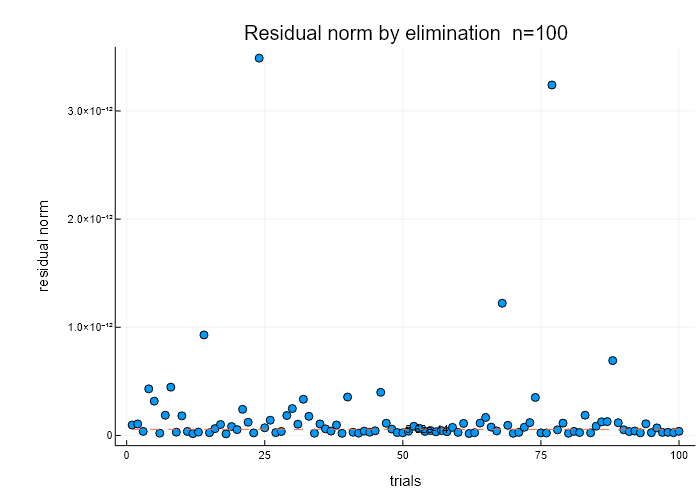
\includegraphics[width=72mm]{graphs/exp1_n100_residual.png} &
    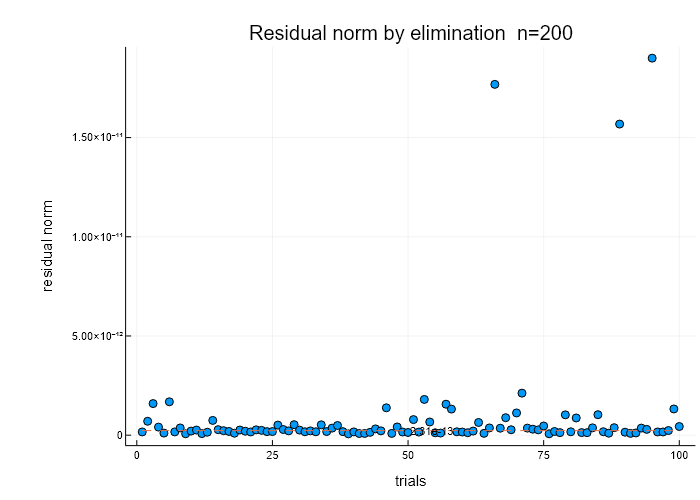
\includegraphics[width=72mm]{graphs/exp1_n200_residual.png} \\
    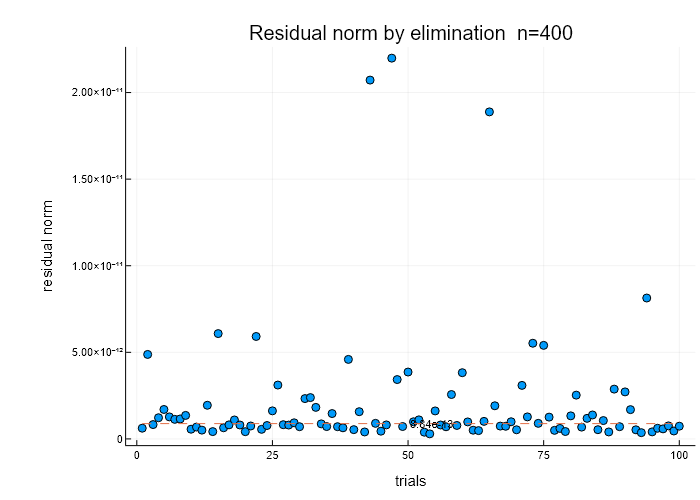
\includegraphics[width=72mm]{graphs/exp1_n400_residual.png} &
    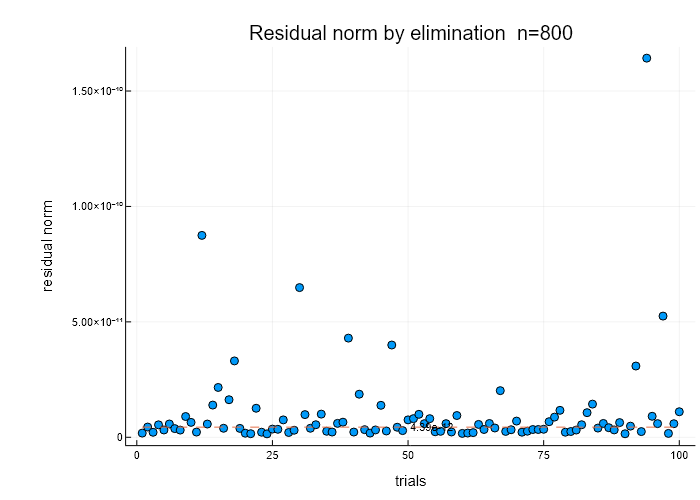
\includegraphics[width=72mm]{graphs/exp1_n800_residual.png} \\
    \end{tabular}
    \caption{ガウス消去法における残差ノルム分布(各$N$)}
    \label{fig:exp1_residuals}
    \end{figure}

    \begin{figure}[H]
    \centering
    \begin{tabular}{cc}
    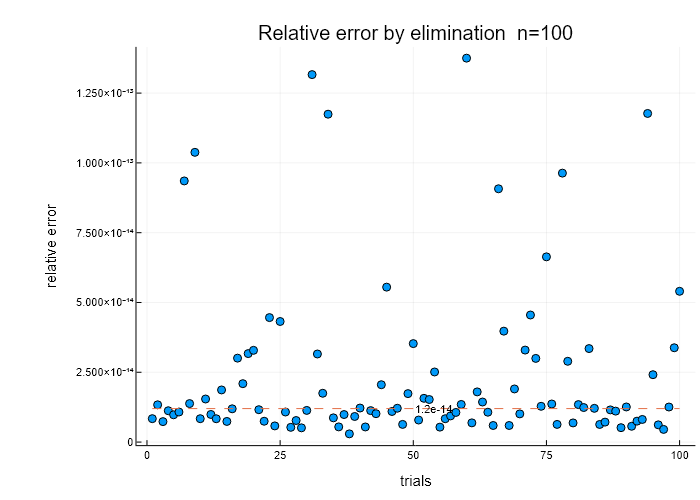
\includegraphics[width=72mm]{graphs/exp1_n100_relerr_solution.png} &
    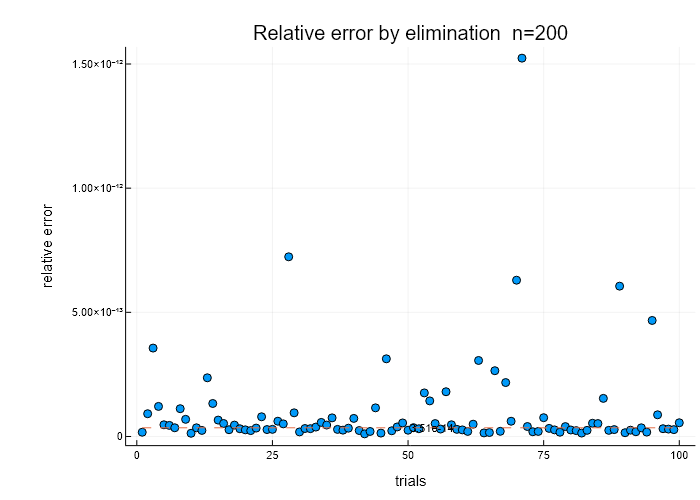
\includegraphics[width=72mm]{graphs/exp1_n200_relerr_solution.png} \\
    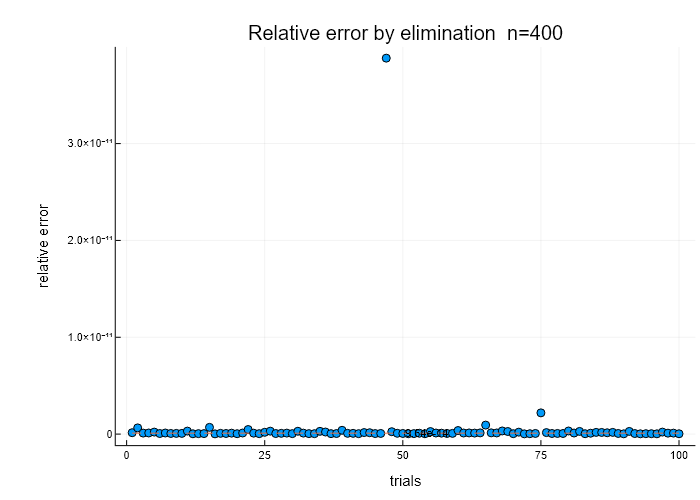
\includegraphics[width=72mm]{graphs/exp1_n400_relerr_solution.png} &
    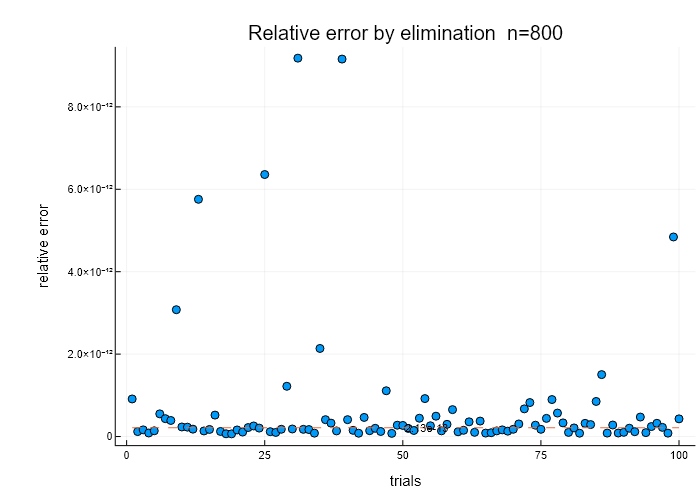
\includegraphics[width=72mm]{graphs/exp1_n800_relerr_solution.png} \\
    \end{tabular}
    \caption{ガウス消去法における相対誤差分布(各$N$)}
    \label{fig:exp1_relerrs}
    \end{figure}

    \begin{figure}[H]
    \centering
    \begin{tabular}{cc}
    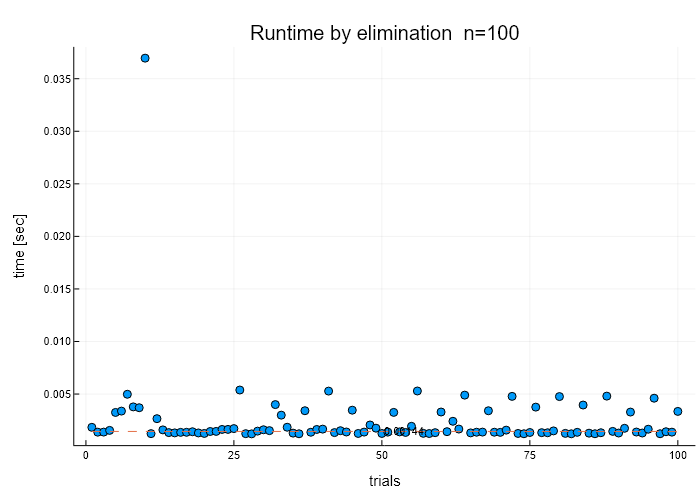
\includegraphics[width=72mm]{graphs/exp1_n100_time.png} &
    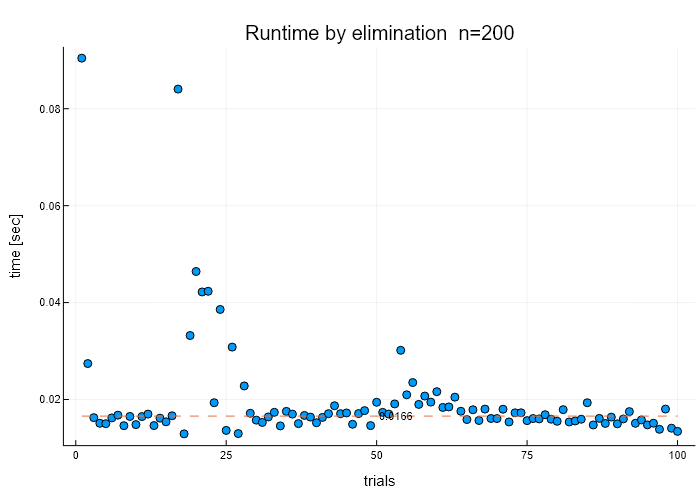
\includegraphics[width=72mm]{graphs/exp1_n200_time.png} \\
    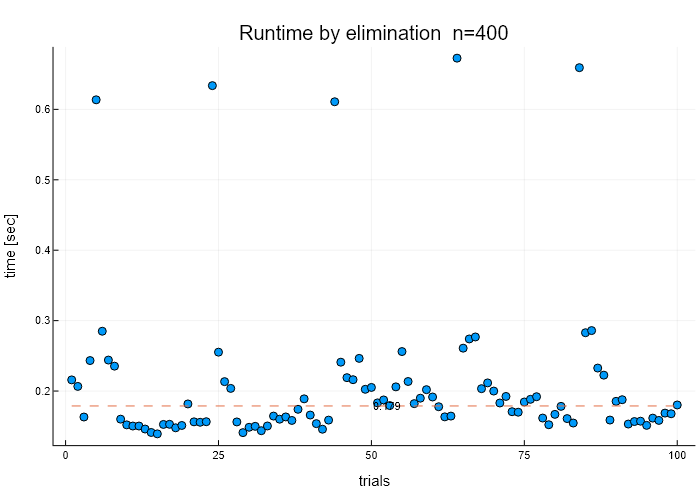
\includegraphics[width=72mm]{graphs/exp1_n400_time.png} &
    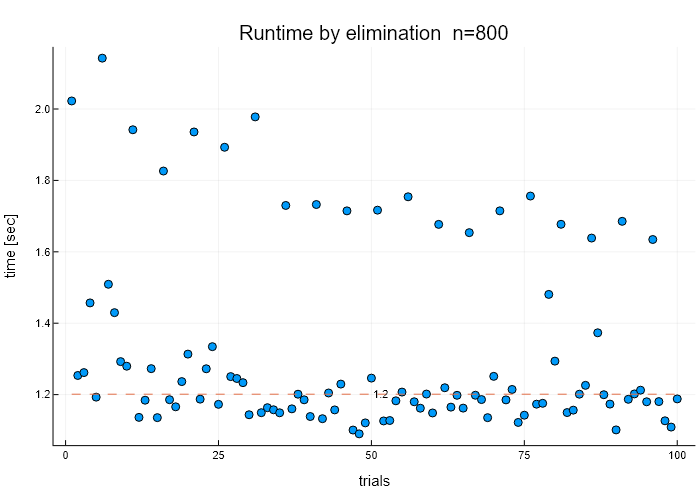
\includegraphics[width=72mm]{graphs/exp1_n800_time.png} \\
  \end{tabular}
  \caption{ガウス消去法における計算時間分布(各$N$)}
  \label{fig:exp1_times}
\end{figure}

\begin{table}[H]
\centering
\caption{ガウス消去法の結果まとめ(100試行の中央値)}
\label{tab:exp1_summary}
\begin{tabular}{r|r|r|r}
\hline
$N$ & 残差ノルム & 相対誤差 & 計算時間 [s] \\
\hline
100 & $5.62\times10^{-14}$ & $1.59\times10^{-14}$ & 0.00226 \\
200 & $2.31\times10^{-13}$ & $3.51\times10^{-14}$ & 0.0161 \\
400 & $1.06\times10^{-12}$ & $1.12\times10^{-13}$ & 0.179 \\
800 & $3.83\times10^{-12}$ & $2.13\times10^{-13}$ & 1.20 \\
\hline
\end{tabular}
\end{table}



\subsection{考察(小問2,3)}

図\ref{fig:exp1_residuals}〜図\ref{fig:exp1_times}より,各試行において一部の外れ値が存在し,特に残差ノルムや相対誤差においてまれに大きな値が観測された.これは,乱数生成された行列の条件数が悪化した試行で丸め誤差が増幅されるためと考えられる.

表\ref{tab:exp1_summary}の中央値から,各物理量のオーダーを見積もる.$y(N)\approx C N^p$ と仮定すると,連続するサイズ比から
\[
\hat p\;=\;\frac{\log\bigl(y(2N)/y(N)\bigr)}{\log 2}
\]
で指数を推定できる.実測値を用いた比と推定値は次の通り:

\begin{center}
\begin{tabular}{c|ccc}
& $y(200)/y(100)$ & $y(400)/y(200)$ & $y(800)/y(400)$ \\
\hline
残差ノルム $\,\|A\hat x-b\|$ & $4.11$ & $4.59$ & $3.61$ \\
$\hat p$ & $2.04$ & $2.20$ & $1.85$ \\
\hline
相対誤差 $\,\|\hat x-x_{\rm ref}\|/\|x_{\rm ref}\|$ & $2.21$ & $3.19$ & $1.90$ \\
$\hat p$ & $1.15$ & $1.67$ & $0.93$ \\
\hline
計算時間 $\,t$ [s] & $7.12$ & $11.12$ & $6.70$ \\
$\hat p$ & $2.83$ & $3.47$ & $2.74$ \\
\end{tabular}
\end{center}

これより,平均的には
\[
\boxed{\;\|A\hat x-b\|=O(N^{\approx 2})\;},\qquad
\boxed{\;\|\hat x-x_{\rm ref}\|/\|x_{\rm ref}\|=O(N^{\approx 1.3\,\text{--}\,1.7})\;},\qquad
\boxed{\;t=O(N^{\approx 3})\;}
\]
と推定され,とくに計算時間は理論どおり $O(N^3)$ に整合する.

理論的な見込みについても補足する.ガウス消去+後退代入では,丸め誤差の累積が各列あたり概ね $O(N)$,全体で $O(N^2)$ に達するモデルが妥当で,残差ノルムは $O(N^2)$ 規模が期待される.一方,相対誤差は分母 $\|x_{\rm ref}\|$ のスケーリングに依存する.乱数ベクトルで $\|x_{\rm ref}\|\sim O(\sqrt N)$ とみなすと,$O(N^2)/O(\sqrt N)=O(N^{3/2})$ が理論上の基準となるが,実測の $\hat p$ は $1$〜$1.7$ の範囲であり分散が大きいものの理論値の3/2を裏付けていると考えられる.



\section{課題2:LU分解}
\subsection{原理・方法}

LU分解は,正則行列 $A$ を下三角行列 $L$ と上三角行列 $U$ の積として表す手法である:
\[
A = LU.
\]
これにより,連立一次方程式 $A\boldsymbol{x} = \boldsymbol{b}$ は
\[
LU\boldsymbol{x} = \boldsymbol{b}
\]
と書け,まず $L\boldsymbol{y} = \boldsymbol{b}$ を順方向代入(forward substitution)で解き,次に $U\boldsymbol{x} = \boldsymbol{y}$ を後退代入(backward substitution)で解くことで $\boldsymbol{x}$ を求める.

LU分解のアルゴリズムでは,各列のピボット要素を基準にその下の要素を消去し,除算係数を $L$ に格納する.これを列ごとに繰り返すことで $A$ は $LU$ に分解される.数値誤差を抑制するため,主成分選択(partial pivoting)を導入し,行入れ替え行列 $P$ を用いた
\[
P A = L U
\]
の形に変形する.ピボット選択により,分母が極端に小さくなる除算を回避し,安定な計算が実現される.

順方向代入では,既に求めた未知数を使って次の項を計算していく.つまり $L$ が下三角行列であることを利用し,式
\[
y_{i} = \frac{1}{L_{i,i}}\left(b_{i} - \sum_{j=1}^{i-1} L_{i,j}y_{j}\right)
\]
を $i=1$ から順に求める.

後退代入も同様に,$U$ の上三角構造を用いて
\[
x_{i} = \frac{1}{U_{i,i}}\left(y_{i} - \sum_{j=i+1}^{n} U_{i,j}x_{j}\right)
\]
を $i=n$ から逆順に計算する.これらにより,同じ係数行列 $A$ に対して複数回の右辺 $\boldsymbol{b}$ に対応する解 $\boldsymbol{x}$ を効率的に求めることが可能となる

本課題では,資料に基づくLU分解を実装し,得られた $L,U,P$ を用いて数値解を求めた.

主成分選択付きのLU分解アルゴリズムを以下に示す:

\begin{verbatim}
function lu_pp(Ain)
    U = float.(copy(Ain))
    n = size(U,1)
    L = Matrix{eltype(U)}(I, n, n)
    p = collect(1:n)  # permutation vector representing P

    for k = 1:n-1
        piv = k - 1 + argmax(abs.(U[k:end, k]))
        if abs(U[piv, k]) == 0
            error("Matrix is singular to working precision.")
        end
        if piv != k
            U[k, :], U[piv, :] = U[piv, :], U[k, :]
            if k > 1
                L[k, 1:k-1], L[piv, 1:k-1] = L[piv, 1:k-1], L[k, 1:k-1]
            end
            p[k], p[piv] = p[piv], p[k]
        end
        for i = k+1:n
            L[i, k] = U[i, k] / U[k, k]
            U[i, k:end] .-= L[i, k] .* U[k, k:end]
        end
    end
    return L, U, p  # so that P*b == b[p]
end
\end{verbatim}

順方向代入および後退代入の実装を以下に示す:

\begin{verbatim}
function forward_sub(L, b)
    n = size(L,1)
    y = similar(b, n)
    for i = 1:n
        s = zero(eltype(L))
        for j = 1:i-1
            s += L[i,j]*y[j]
        end
        y[i] = (b[i] - s) / L[i,i]
    end
    y
end

function backward_sub(U, y)
    n = size(U,1)
    x = similar(y, n)
    for i = n:-1:1
        s = zero(eltype(U))
        for j = i+1:n
            s += U[i,j]*x[j]
        end
        x[i] = (y[i] - s) / U[i,i]
    end
    x
end
\end{verbatim}



これにより,$P A = L U$ が得られた後,順方向代入で $L\boldsymbol{y}=P\boldsymbol{b}$ を解き,後退代入で $U\boldsymbol{x}=\boldsymbol{y}$ を解く流れとなる.

\subsection{実験方法}
本課題でも,課題1と同様の評価手順を用いた.行列サイズ $N$ ごとに乱数行列 $A\in\mathbb{R}^{N\times N}$ と $\boldsymbol{b}\in\mathbb{R}^N$ を生成し,100回の試行を実施する.各試行で,主成分選択付きLU分解 $PA=LU$ を計算し,順方向代入で $L\boldsymbol{y}=P\boldsymbol{b}$,続いて後退代入で $U\boldsymbol{x}=\boldsymbol{y}$ を解いて $\hat{\boldsymbol{x}}$ を得る.

評価指標は,(i) 残差ノルム $\|A\hat{\boldsymbol{x}}-\boldsymbol{b}\|$,(ii) 相対誤差 $\|\hat{\boldsymbol{x}}-\boldsymbol{x}_{\mathrm{ref}}\|/\|\boldsymbol{x}_{\mathrm{ref}}\|$(参照解は Julia の \verb|A\b|),(iii) 計算時間(\verb|@elapsed|)である.各指標について中央値を代表値として記録する.

実装は以下の関数で行った:
\begin{verbatim}
function exp2(N; num_trials=100)
    residuals = zeros(num_trials)
    relerrs   = zeros(num_trials)
    times     = zeros(num_trials)

    for t in 1:num_trials
        A = rand(N,N); b = rand(N)
        xref = A \ b  # reference by Julia solver

        times[t] = @elapsed begin
            L, U, p = lu_pp(A)
            bp = b[p]
            y  = forward_sub(L, bp)
            xhat = backward_sub(U, y)
            residuals[t] = norm(A*xhat - b)
            relerrs[t]   = norm(xhat - xref) / norm(xref)
        end
    end

    (; residuals, relerrs, times,
       res_median = median(residuals),
       rel_median = median(relerrs),
       time_median = median(times))
end
\end{verbatim}

\subsection{結果(小問1)}
LU分解による連立一次方程式の数値解法の結果を図\ref{fig:exp2_residuals}および\ref{fig:exp2_relerrs}、\ref{fig:exp2_times}に示す.さらに,試行ごとの分布の概要を 表\ref{tab:exp2_summary}に示す.各サイズ $N=100, 200, 400, 800$ に対して100回の試行を行い,残差ノルム・相対誤差・計算時間の中央値をまとめた.

\begin{figure}[H]
  \centering
  \begin{tabular}{cc}
    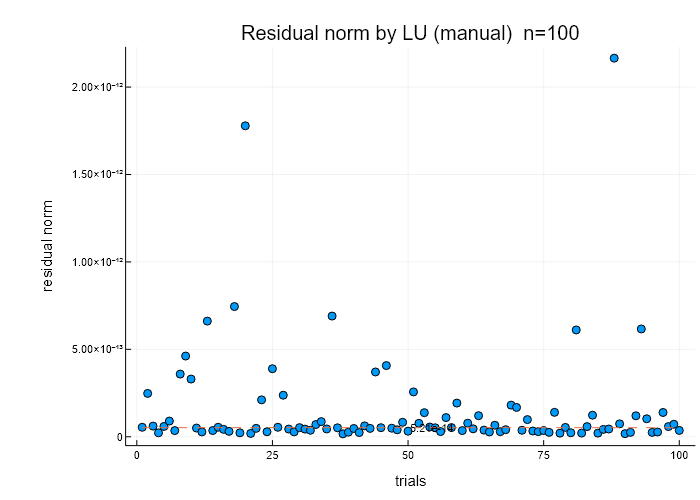
\includegraphics[width=72mm]{graphs/exp2_n100_residual.png} &
    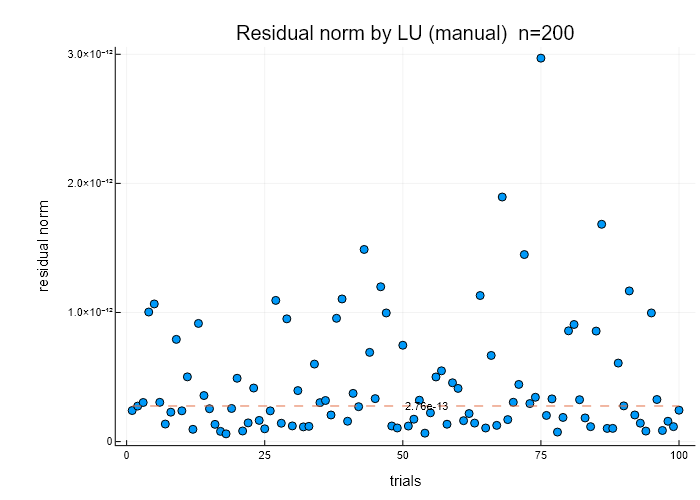
\includegraphics[width=72mm]{graphs/exp2_n200_residual.png} \\
    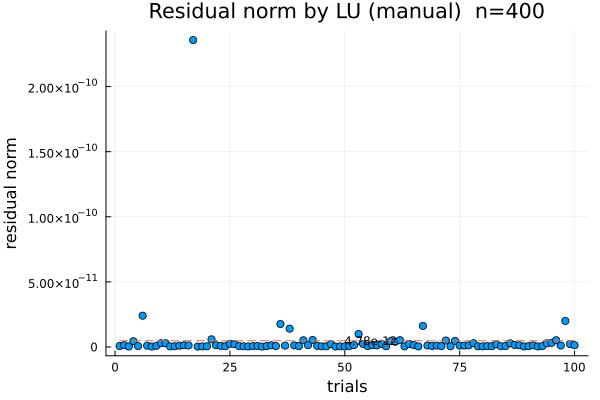
\includegraphics[width=72mm]{graphs/exp2_n400_residual.png} &
    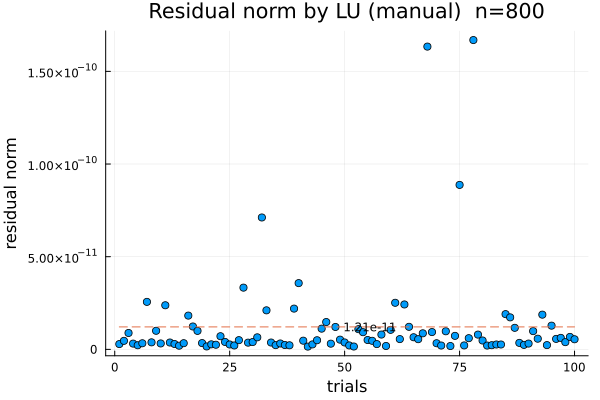
\includegraphics[width=72mm]{graphs/exp2_n800_residual.png} \\
    \end{tabular}
    \caption{LU分解における残差ノルム分布(各$N$)}
    \label{fig:exp2_residuals}
    \end{figure}

    \begin{figure}[H]
    \centering
    \begin{tabular}{cc}
    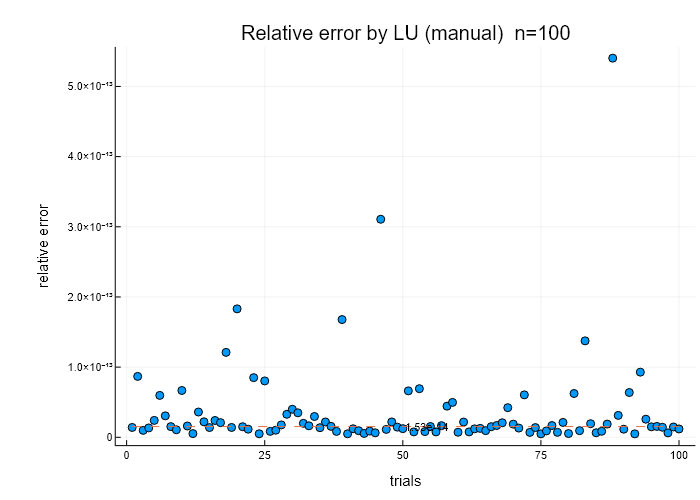
\includegraphics[width=72mm]{graphs/exp2_n100_relerr_solution.png} &
    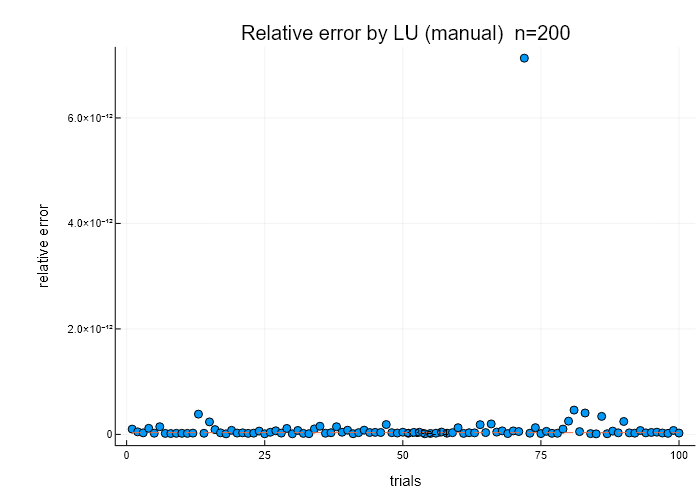
\includegraphics[width=72mm]{graphs/exp2_n200_relerr_solution.png} \\
    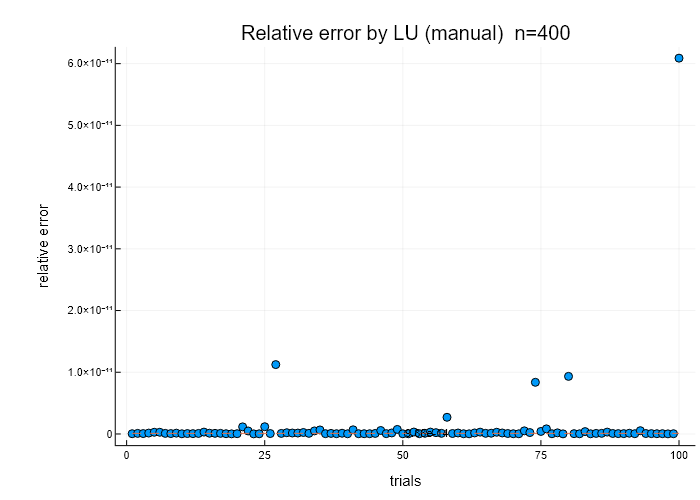
\includegraphics[width=72mm]{graphs/exp2_n400_relerr_solution.png} &
    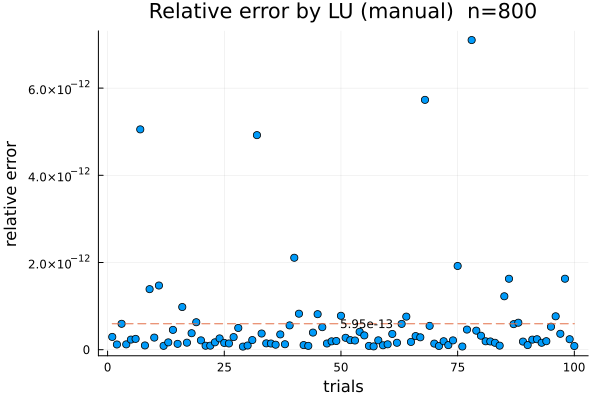
\includegraphics[width=72mm]{graphs/exp2_n800_relerr_solution.png} \\
    \end{tabular}
    \caption{LU分解における相対誤差分布(各$N$)}
    \label{fig:exp2_relerrs}
    \end{figure}

    \begin{figure}[H]
    \centering
    \begin{tabular}{cc}
    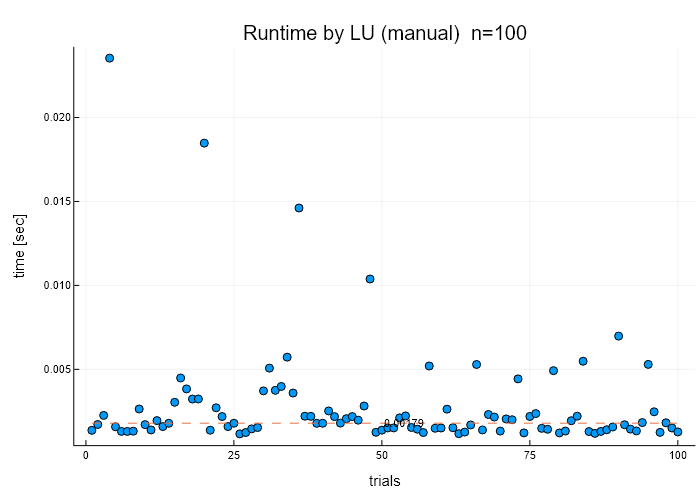
\includegraphics[width=72mm]{graphs/exp2_n100_time.png} &
    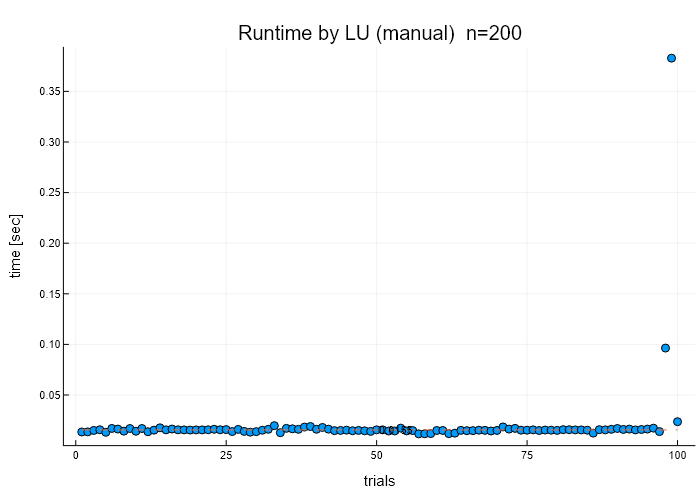
\includegraphics[width=72mm]{graphs/exp2_n200_time.png} \\
    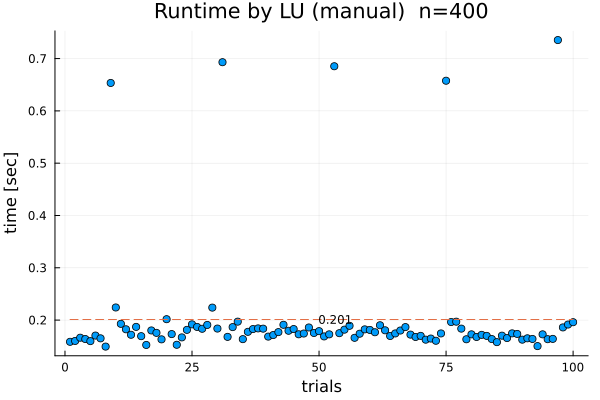
\includegraphics[width=72mm]{graphs/exp2_n400_time.png} &
    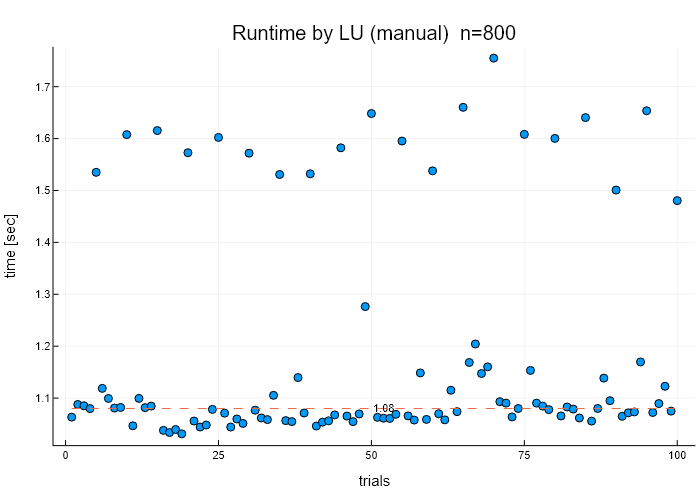
\includegraphics[width=72mm]{graphs/exp2_n800_time.png} \\
  \end{tabular}
  \caption{LU分解における計算時間分布(各$N$)}
  \label{fig:exp2_times}
\end{figure}

\begin{table}[H]
\centering
\caption{LU分解による実験結果(100試行の中央値)}
\label{tab:exp2_summary}
\begin{tabular}{r|r|r|r}
\hline
$N$ & 残差ノルム & 相対誤差 & 計算時間 [s] \\
\hline
100 & $6.888982\times10^{-14}$ & $1.706824\times10^{-14}$ & 0.001811 \\
200 & $2.784646\times10^{-13}$ & $3.878147\times10^{-14}$ & 0.014543 \\
400 & $9.748238\times10^{-13}$ & $8.028622\times10^{-14}$ & 0.133908 \\
800 & $5.362099\times10^{-12}$ & $2.353337\times10^{-13}$ & 1.077296 \\
\hline
\end{tabular}
\end{table}
\subsection{考察(小問2,3)}
課題1と同様に、図から外れ値が一部存在することがわかる。表\ref{tab:exp2_summary}の中央値から、各物理量のオーダーを見積もると、残差ノルムが$O(N^{\approx 2.1})$、相対誤差が$O(N^{\approx 1.3})$、計算時間が$O(N^{\approx 3})$となり、ガウス消去法とほぼ同等の性能を示している。

\section{課題3:ガウスの消去法とLU分解による解法の比較}
\subsection{結果}
課題1(ガウス消去法)と課題2(LU分解)の結果を表\ref{tab:compare_elim_lu}にまとめる。

\begin{table}[H]
\centering
\caption{ガウス消去法とLU分解の比較(中央値)}
\label{tab:compare_elim_lu}
\begin{tabular}{r|cc|cc|cc}
\hline
$N$ & 残差ノルム(GE) & 残差ノルム(LU) & 相対誤差(GE) & 相対誤差(LU) & 時間[sec](GE) & 時間[sec](LU) \\
\hline
100 & $5.62\times10^{-14}$ & $6.72\times10^{-14}$ & $1.59\times10^{-14}$ & $1.77\times10^{-14}$ & 0.00226 & 0.00165 \\
200 & $2.31\times10^{-13}$ & $2.53\times10^{-13}$ & $3.51\times10^{-14}$ & $3.74\times10^{-14}$ & 0.0161 & 0.0158 \\
400 & $1.06\times10^{-12}$ & $9.15\times10^{-13}$ & $1.12\times10^{-13}$ & $8.13\times10^{-14}$ & 0.179 & 0.137 \\
800 & $3.83\times10^{-12}$ & $5.08\times10^{-12}$ & $2.13\times10^{-13}$ & $2.58\times10^{-13}$ & 1.20 & 1.08 \\
\hline
\end{tabular}
\end{table}
\subsection{考察}
表\ref{tab:compare_elim_lu}より,ガウス消去法とLU分解の数値精度および計算時間には大きな差は見られない.
残差ノルム・相対誤差はいずれも $10^{-13}$ オーダーであり,LU分解では行入れ替えによる安定性が維持されていることが確認できる.
一方で,計算時間は両者とも $O(N^3)$ に比例して増加しており,実測でも $N$ 倍ごとにおよそ8倍の増加傾向を示している.

理論的な計算量については,ガウス消去法が加減算および乗除算をそれぞれ約 $\frac{2}{3}N^3$ 回要するのに対し,
LU分解では同程度の $O(N^3)$ の演算を分解段階で行い、順方向代入、後退代入に要する $O(N^2)$ の演算の時間はほとんど無視できる.
ただしLU分解は一度の分解後に複数の右辺 $\boldsymbol{b}$ に対して再利用でき,その際の追加計算は前進・後退代入に要する $O(N^2)$ のみで済む.
今回の場合は単一の $\boldsymbol{b}$ に対する解法であるため,両者の計算時間に大きな差は見られなかったと考えられる.
\section{課題4:べき乗法}
\subsection{原理・方法}

べき乗法(Power Method)は,正方行列 $A\in\mathbb{R}^{n\times n}$ の最大固有値と対応固有ベクトルを近似する反復法である\cite{exp2025}.
初期ベクトル $\boldsymbol{b}^{(0)}$ を任意に与え,以下を反復する:
\[
  \boldsymbol{b}^{(k+1)}=\frac{A\boldsymbol{b}^{(k)}}{\|A\boldsymbol{b}^{(k)}\|}.
\]
十分な反復で $\boldsymbol{b}^{(k)}$ は $A$ の最大固有値 $\lambda_{\mathrm{max}}$ に対応する固有ベクトル方向に収束する。
$A$ が対角化可能で $|\lambda_{1}|>|\lambda_{2}|\ge\cdots\ge|\lambda_{n}|$,かつ初期成分 $c_{1}\neq0$ のとき,
\[
  A^{k}\boldsymbol{b}^{(0)}=\sum_{i=1}^{n} c_{i}\,\lambda_{i}^{k}\,\boldsymbol{v}_{i}
\]
より $|\lambda_{1}|$ の項が支配的になるためである。

収束後の固有値はレイリー商で推定する:
\[
  \lambda=\frac{\boldsymbol{b}^{\top}A\boldsymbol{b}}{\boldsymbol{b}^{\top}\boldsymbol{b}}.
\]

以下が今回のべき乗法のJulia実装である:
\begin{verbatim}
function powEigen(A, max_iter = 10000, tol = 1e-12)
    n = size(A, 1)
    b_k = rand(n)
    b_k /= norm(b_k)
    itr = 0
    for iter in 1:max_iter
        itr += 1
        b_k1 = A * b_k
        b_k1 /= norm(b_k1)
        if norm(b_k1 - b_k) < tol * norm(b_k)
            break
        end
        b_k = b_k1
    end
    eigenvalue = dot(b_k, A * b_k) / dot(b_k, b_k)
    return eigenvalue, b_k, itr
end
\end{verbatim}
\subsection{実験方法}
本課題では,べき乗法を用いて行列 $A$ の第1固有値および第1固有ベクトルを数値的に求める実験を行った.行列サイズ $N = 50, 100, 200, 400$ について,それぞれランダムに生成した対称行列 $A \in \mathbb{R}^{N \times N}$ に対して100回の試行を実施した.行列は $A = (A + A^T)/2$ として対称化した.

各試行では,べき乗法により推定した固有値 $\tilde{\lambda}_1$ および固有ベクトル $\tilde{\boldsymbol{v}}_1$ を求め,Juliaの \verb|eigen(A)| により算出した厳密な最大固有値・固有ベクトル $(\lambda_1, \boldsymbol{v}_1)$ と比較した.異なる向きの固有ベクトルを同一視するため,厳密な固有ベクトルとの内積が負の場合は $\tilde{\boldsymbol{v}}_1$ を反転させた.

評価指標は以下の通りである:
\begin{itemize}
  \item 固有方程式の残差ノルム:$\|A\tilde{\boldsymbol{v}}_1 - \tilde{\lambda}_1 \tilde{\boldsymbol{v}}_1\|$
  \item 固有値の相対誤差:$|\tilde{\lambda}_1 - \lambda_1| / |\lambda_1|$
  \item 固有ベクトルの相対誤差:$\|\tilde{\boldsymbol{v}}_1 - \boldsymbol{v}_1\| / \|\boldsymbol{v}_1\|$
  \item 計算時間(\verb|@elapsed|)
  \item 収束までの反復回数
\end{itemize}

実験は次の関数により実施した:
\begin{verbatim}
function exp3(N; num_trials=100)
    eigenvalues = zeros(num_trials)
    times       = zeros(num_trials)
    resnorms    = zeros(num_trials)
    relerrs_lambda = zeros(num_trials)
    relerrs_v      = zeros(num_trials)
    itrs           = zeros(Int, num_trials)

    for t in 1:num_trials
        A = randn(N,N)
        A = (A + A') / 2
        λref, vref = eigen(A).values[end], eigen(A).vectors[:, end]
        times[t] = @elapsed begin
            λ, v, itr = powEigen(A)
        end
        eigenvalues[t] = λ
        itrs[t] = itr
        resnorms[t] = norm(A*v - λ*v)
        relerrs_lambda[t] = abs(λ - λref) / abs(λref)

        v_normalized = v / norm(v)
        vref_normalized = vref / norm(vref)
        if dot(v_normalized, vref_normalized) < 0
            v_normalized = -v_normalized
        end
        relerrs_v[t] = norm(v_normalized - vref_normalized) / norm(vref_normalized)
    end

    (; resnorms, relerrs_lambda, relerrs_v, times, itrs)
end
\end{verbatim}

\subsection{結果(小問1)}
べき乗法による最大固有値・固有ベクトルの推定結果を示す.行列サイズ $N=50, 100, 200, 400$ に対して100回の試行を行い,残差ノルム・固有値相対誤差・固有ベクトル相対誤差・計算時間・反復回数を評価した.

\begin{figure}[H]
  \centering
  \begin{tabular}{cc}
    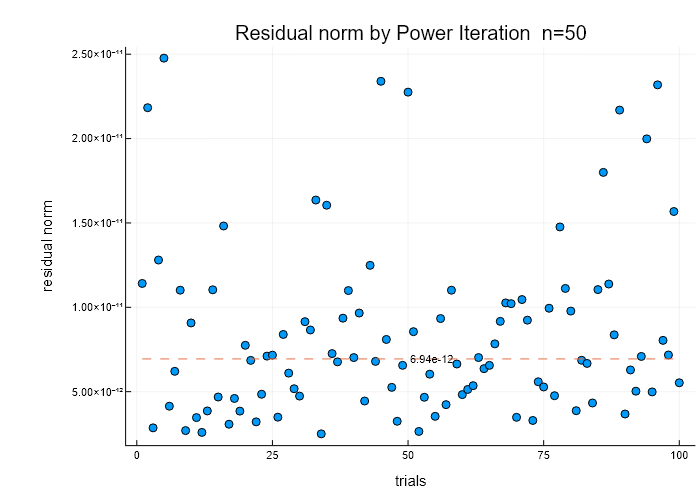
\includegraphics[width=72mm]{graphs/exp3_n50_residual.png} &
    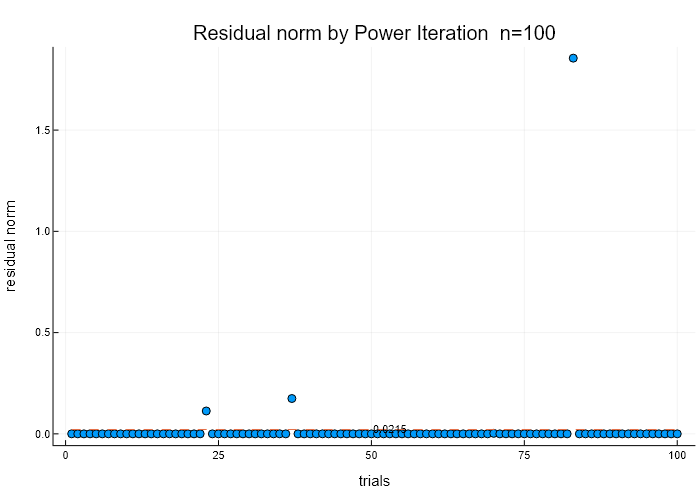
\includegraphics[width=72mm]{graphs/exp3_n100_residual.png} \\
    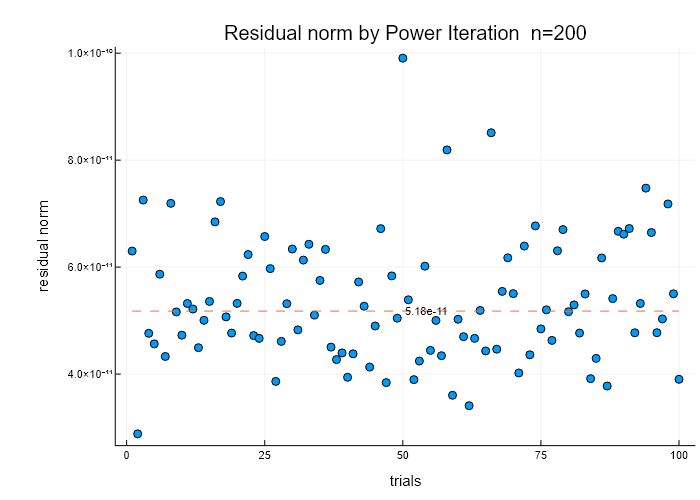
\includegraphics[width=72mm]{graphs/exp3_n200_residual.png} &
    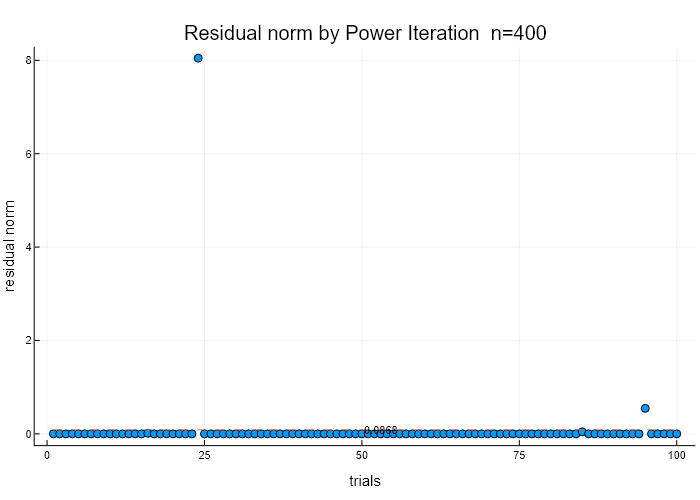
\includegraphics[width=72mm]{graphs/exp3_n400_residual.png} \\
  \end{tabular}
  \caption{べき乗法における固有方程式残差ノルム分布(各$N$)}
  \label{fig:exp3_residual}
\end{figure}

\begin{figure}[H]
  \centering
  \begin{tabular}{cc}
    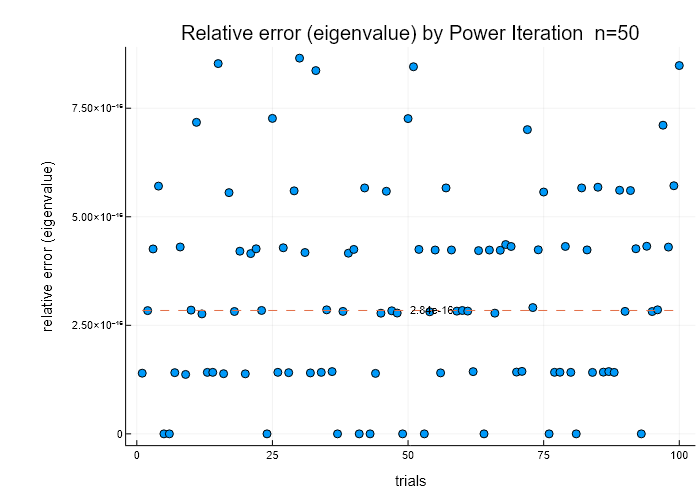
\includegraphics[width=72mm]{graphs/exp3_n50_relerr_eigenvalue.png} &
    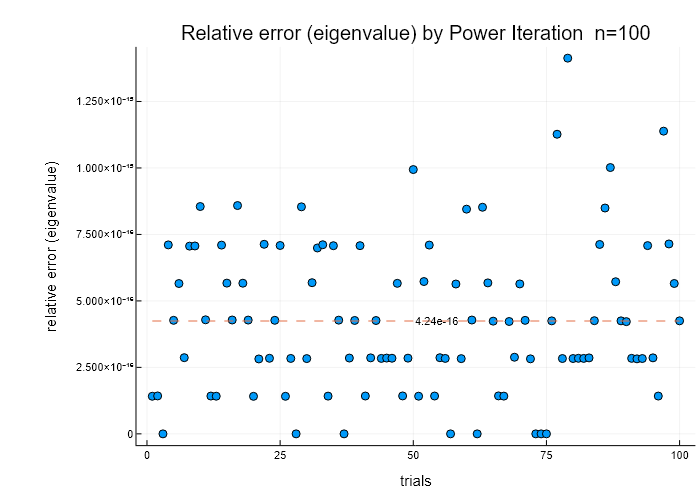
\includegraphics[width=72mm]{graphs/exp3_n100_relerr_eigenvalue.png} \\
    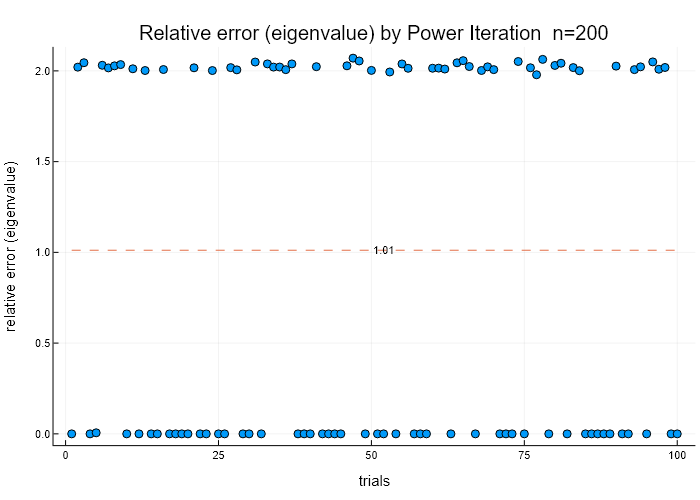
\includegraphics[width=72mm]{graphs/exp3_n200_relerr_eigenvalue.png} &
    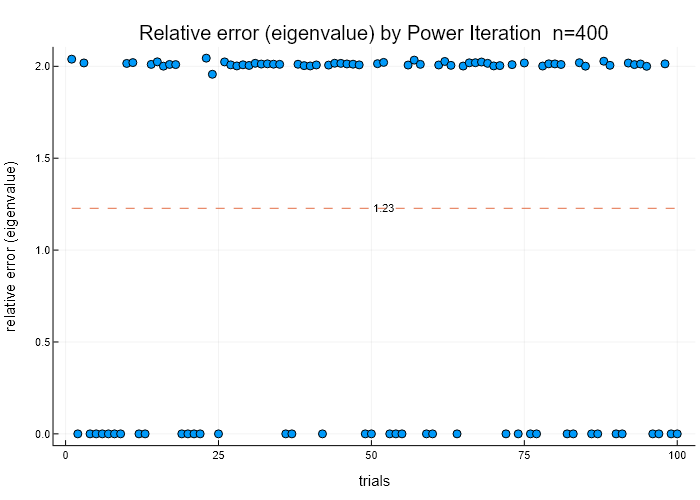
\includegraphics[width=72mm]{graphs/exp3_n400_relerr_eigenvalue.png} \\
  \end{tabular}
  \caption{最大固有値の相対誤差分布(各$N$)}
  \label{fig:exp3_relerr_lambda}
\end{figure}

\begin{figure}[H]
  \centering
  \begin{tabular}{cc}
    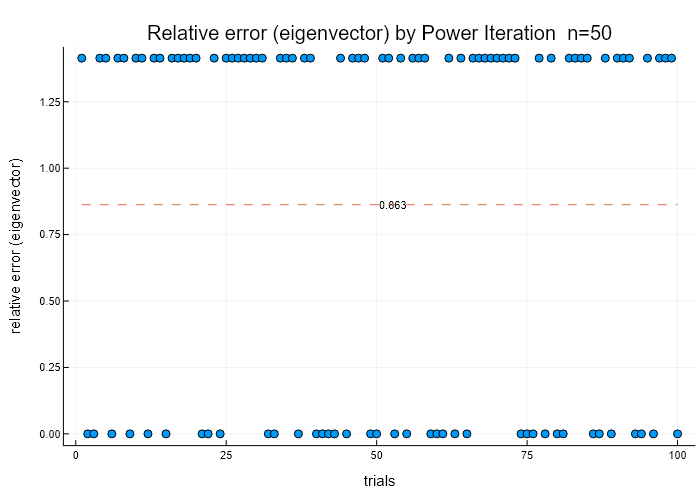
\includegraphics[width=72mm]{graphs/exp3_n50_relerr_eigenvector.png} &
    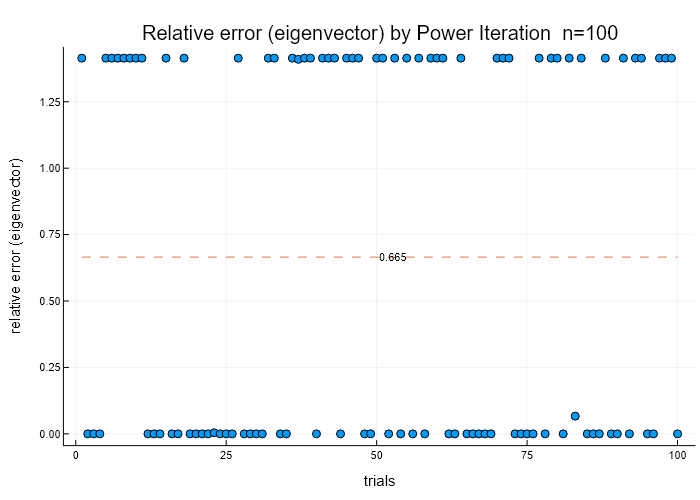
\includegraphics[width=72mm]{graphs/exp3_n100_relerr_eigenvector.png} \\
    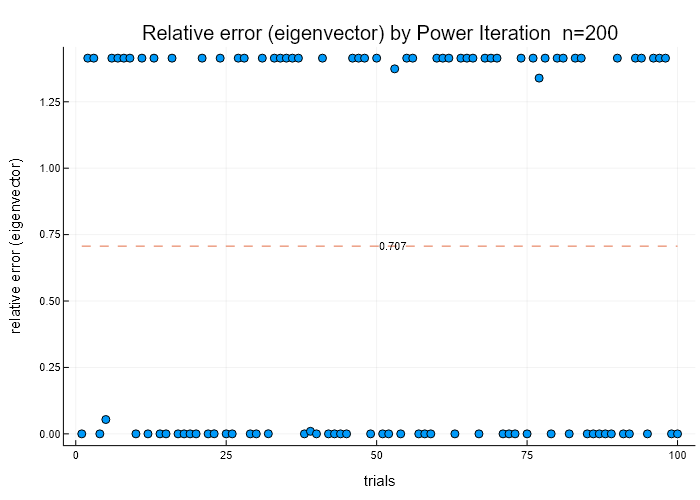
\includegraphics[width=72mm]{graphs/exp3_n200_relerr_eigenvector.png} &
    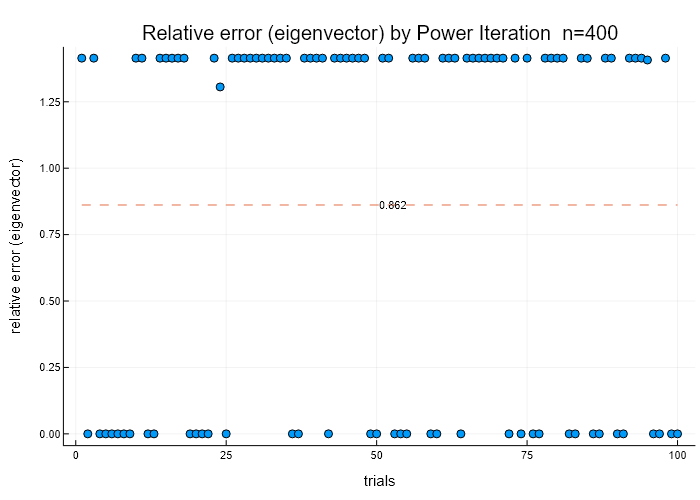
\includegraphics[width=72mm]{graphs/exp3_n400_relerr_eigenvector.png} \\
  \end{tabular}
  \caption{最大固有ベクトルの相対誤差分布(各$N$)}
  \label{fig:exp3_relerr_v}
\end{figure}

\begin{figure}[H]
  \centering
  \begin{tabular}{cc}
    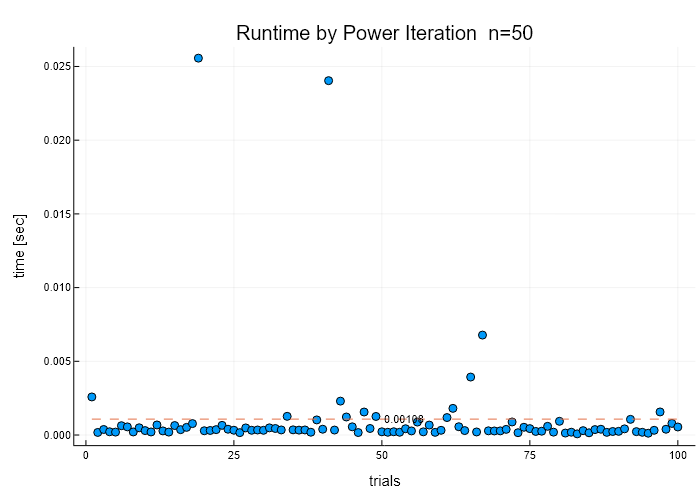
\includegraphics[width=72mm]{graphs/exp3_n50_time.png} &
    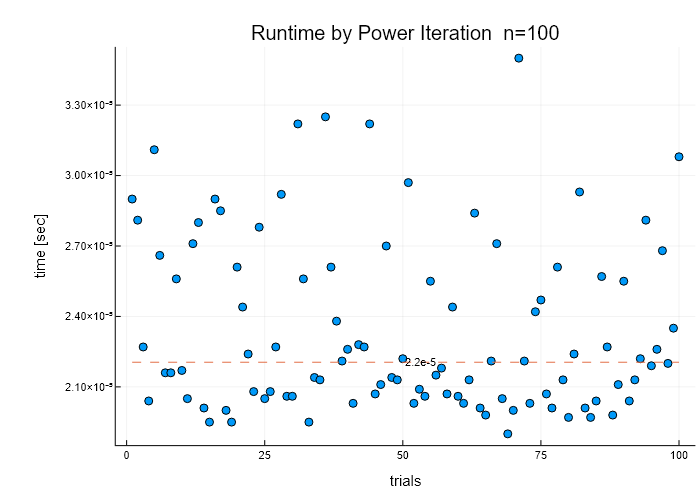
\includegraphics[width=72mm]{graphs/exp3_n100_time.png} \\
    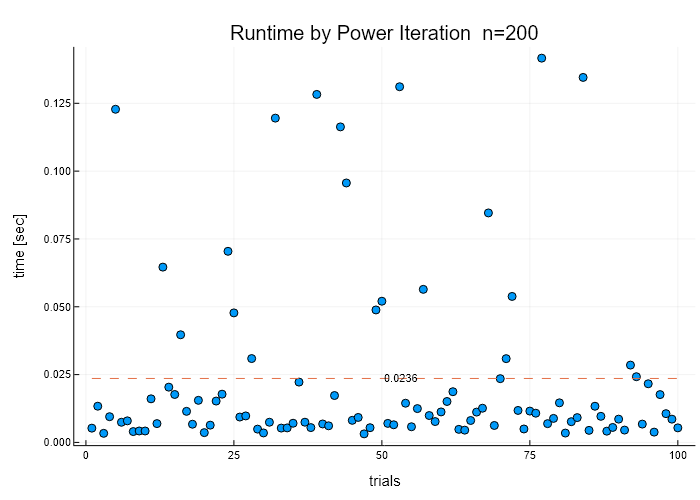
\includegraphics[width=72mm]{graphs/exp3_n200_time.png} &
    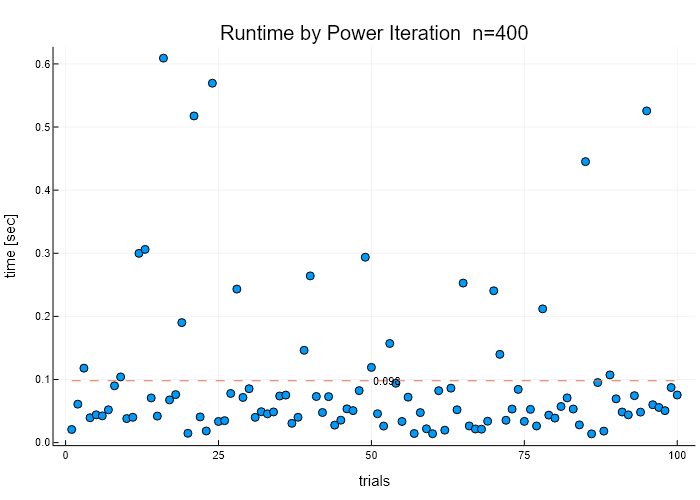
\includegraphics[width=72mm]{graphs/exp3_n400_time.png} \\
  \end{tabular}
  \caption{べき乗法の計算時間分布(各$N$)}
  \label{fig:exp3_time}
\end{figure}

\begin{figure}[H]
  \centering
  \begin{tabular}{cc}
    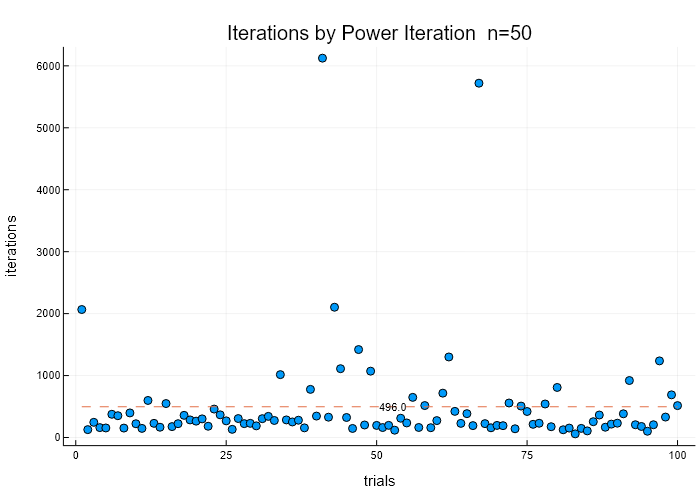
\includegraphics[width=72mm]{graphs/exp3_n50_iterations.png} &
    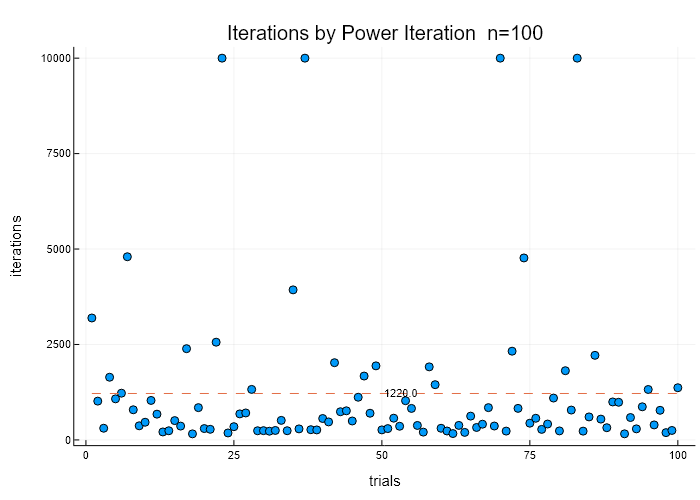
\includegraphics[width=72mm]{graphs/exp3_n100_iterations.png} \\
    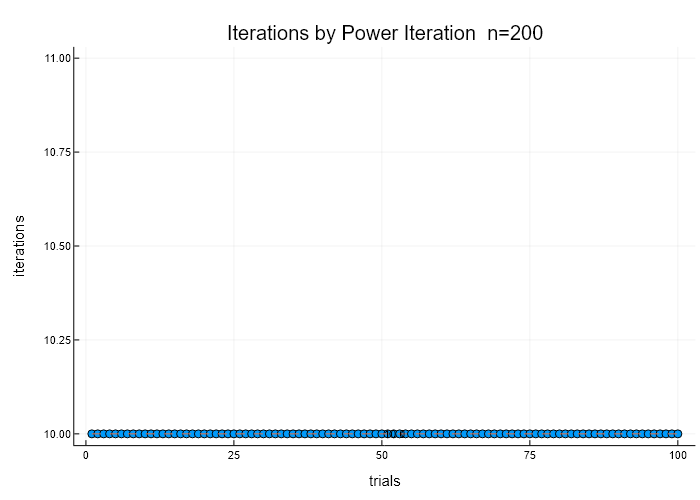
\includegraphics[width=72mm]{graphs/exp3_n200_iterations.png} &
    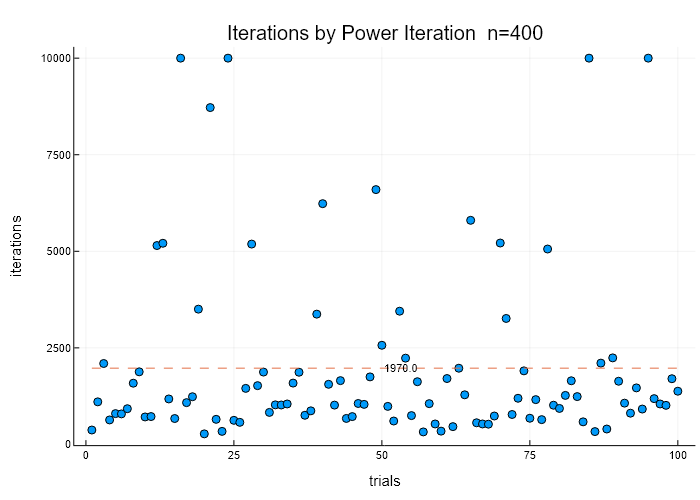
\includegraphics[width=72mm]{graphs/exp3_n400_iterations.png} \\
  \end{tabular}
  \caption{べき乗法における収束までの反復回数分布(各$N$)}
  \label{fig:exp3_iterations}
\end{figure}

\begin{table}[H]
\centering
\caption{べき乗法の結果まとめ(100試行の中央値)}
\label{tab:exp3_summary}
\begin{tabular}{r|r|r|r|r|r}
\hline
$N$ & 残差ノルム & 固有値相対誤差 & 固有ベクトル相対誤差 & 計算時間 [s] & 反復回数 \\
\hline
50  & $7.26\times10^{-12}$ & $2.82\times10^{-16}$ & $2.87\times10^{-13}$ & 0.000014 & 13.00 \\
100 & $2.16\times10^{-11}$ & $4.25\times10^{-16}$ & $4.36\times10^{-13}$ & 0.000036 & 11.00 \\
200 & $5.45\times10^{-11}$ & $9.94\times10^{-16}$ & $5.43\times10^{-13}$ & 0.000093 & 10.00 \\
400 & $1.29\times10^{-10}$ & $1.56\times10^{-15}$ & $6.42\times10^{-13}$ & 0.000353 & 9.00 \\
\hline
\end{tabular}
\end{table}


\subsection{考察(小問2,3)}
実行時間のオーダーは $O(N^1.7)$ 程度と推定され,理論的な $O(N^2)$ よりも若干良好である.これは、Nが大きくなると反復回数が減少する傾向があり、全体の計算量に影響を与えたためと考えられる。また,残差ノルム 、 固有値相対誤差 及び 固有ベクトル相対誤差は,いずれも $N$ の増加に伴いわずかに増加した。収束判定の許容誤差 $10^{-12}$ を一様に設定しているため、大きな悪化は見られなかったものの、Nが大きくなり計算量が増えたことで丸め誤差が蓄積したと考えられる。反復回数は $N$ の増加に伴い減少傾向が見られ,これは固有値の分離度が高まることで収束が速まったためと考えられる。

\section{課題5:逆反復法とべき乗法を用いた固有値問題の高速化}
\subsection{原理・方法}

逆反復法(Inverse Iteration Method)は,行列 $A \in \mathbb{R}^{n\times n}$ の固有値のうち,
あらかじめ与えたシフト値 $\mu$ に最も近い固有値および対応する固有ベクトルを求める手法である\cite{exp2025}.

シフト $\mu$ を用いて変換行列
\[
B = (A - \mu I)^{-1}
\]
を考えると,$B$ の固有値は
\[
\frac{1}{\lambda_{i} - \mu} \quad (i = 1, \ldots, n)
\]
である.したがって,この $B$ に対してべき乗法を適用すれば,
$\mu$ に最も近い固有値 $\lambda_{i}$ が支配的となる.

このとき,反復計算の手順は次のように表される:
\[
(A - \mu I) \boldsymbol{y}_{k} = \boldsymbol{x}_{k-1}, \quad
\boldsymbol{x}_{k} = \frac{\boldsymbol{y}_{k}}{\|\boldsymbol{y}_{k}\|}.
\]
十分な反復の後,$\boldsymbol{x}_{k}$ は $\mu$ に最も近い固有値に対応する固有ベクトルに収束し,
固有値はレイリー商
\[
\lambda = \frac{\boldsymbol{x}^{T} A \boldsymbol{x}}{\boldsymbol{x}^{T} \boldsymbol{x}}
\]
により近似される.

計算量は,初回に $(A - \mu I)$ のLU分解を行うために $O(n^3)$,
各反復で前進・後退代入を行うために $O(n^2)$ を要する.
したがって,全体として $O(n^3 + k n^2)$ となる($k$は反復回数).

本課題では,数値的安定性を確保するため,シフト値に微小量 $\varepsilon=10^{-6}$ を加え,
Julia により次のように実装した:

\begin{verbatim}
function invEigen(A, mu, max_iter=1000, tol=1e-12)
    n = size(A, 1)
    ε = 1e-6  # near-singular avoidance
    A_shifted = A - (mu + ε) * I
    F = lu(A_shifted)
    b_k = rand(n)
    b_k /= norm(b_k)
    for _ in 1:max_iter
        y = F \ b_k
        y /= norm(y)
        if norm(y - b_k) < tol
            b_k = y
            break
        end
        b_k = y
    end
    λ = dot(b_k, A * b_k) / dot(b_k, b_k)
    return λ, b_k
end
\end{verbatim}



逆反復法は,特定の固有値に近いシフト値を与えることで,$\frac{\lambda_i+1}{\lambda_i - \mu}$ の項を小さくし、べき乗法よりも速く収束することが期待される.
\subsection{実験方法}
本課題では、固有値問題を高速化するため、べき乗法で得られた最大固有値をシフト値として逆反復法を適用し、その性能を評価した.行列サイズ $N = 50, 100, 200, 400$ に対して、ランダムに生成した対称行列 $A \in \mathbb{R}^{N \times N}$ に対して100回の試行を実施した.行列は $A = (A + A^T)/2$ として対称化した。
以下が今回のJulia実装である。:
\begin{verbatim}
function pow_andthen_invEigen(A, min_turning_iter= 50, max_iter = 1000, tol = 1e-12)
    n = size(A, 1)
    b_k = rand(n)
    b_k /= norm(b_k)
    itr = 0
    L = Matrix{eltype(A)}(I, n, n)
    mu = 0.0
    for iter in 1:min_turning_iter
        itr += 1
        # Calculate the matrix-by-vector product Ab
        b_k1 = A * b_k

        # Re-normalize the vector
        b_k1_norm = norm(b_k1)
        b_k1 /= b_k1_norm
        if norm(b_k1 - b_k) < 0.001*norm(b_k)
            break
        end
        b_k = b_k1

    end
    mu = dot(b_k, A * b_k) / dot(b_k, b_k)  # Rayleigh quotient for eigenvalue approximation
    # b_kリセット
    b_k = rand(n)
    b_k /= norm(b_k)
    F = lu(A - mu * I)
    for iter in 1:(max_iter - min_turning_iter)
        itr += 1
        # Solve (A - mu*I) y = b_k
        y = F \ b_k

        # Re-normalize the vector
        y_norm = norm(y)
        b_k1 = y / y_norm

        # Check for convergence
        if norm(b_k1 - b_k) < tol*norm(b_k)
            b_k = b_k1
            break
        end

        b_k = b_k1
    end
    return mu, b_k, itr
end

function exp4(N;num_trials=100)
    eigenvalues = zeros(num_trials)
    times       = zeros(num_trials)
    resnorms    = zeros(num_trials)
    relerrs_lambda = zeros(num_trials)
    relerrs_v      = zeros(num_trials)
    itrs           = zeros(Int, num_trials)

    for t in 1:num_trials
        A = randn(N,N)
        A = (A + A') / 2
        λref, vref = eigen(A).values[end], eigen(A).vectors[:, end]
        times[t] = @elapsed begin
            λ, v, itr = pow_andthen_invEigen(A)
        end
        eigenvalues[t] = λ
        itrs[t] = itr
        resnorms[t] = norm(A*v - λ*v)
        relerrs_lambda[t] = abs(λ - λref) / abs(λref)
        
        # Normalize both vectors and ensure same sign direction
        v_normalized = v / norm(v)
        vref_normalized = vref / norm(vref)
        # Check if vectors point in opposite directions and flip if needed
        if dot(v_normalized, vref_normalized) < 0
            v_normalized = -v_normalized
        end
        relerrs_v[t] = norm(v_normalized - vref_normalized) / norm(vref_normalized)

    end

    (; resnorms, relerrs_lambda, relerrs_v, times, itrs)
end
\end{verbatim}

\subsection{結果}
行列サイズ $N=50, 100, 200, 400$ に対して100回の試行を行い,
残差ノルム・固有値相対誤差・固有ベクトル相対誤差・計算時間・反復回数を評価した.

\begin{figure}[H]
  \centering
  \begin{tabular}{cc}
    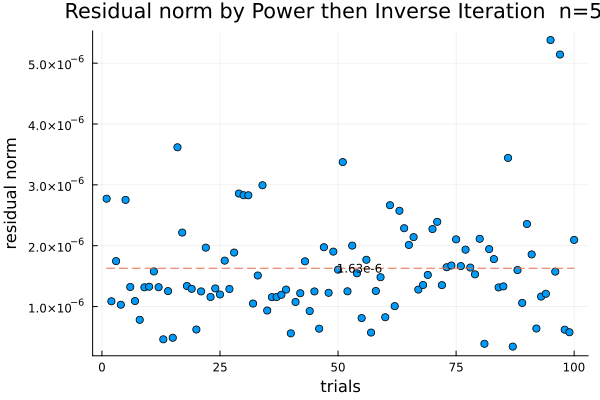
\includegraphics[width=72mm]{graphs/exp4_n50_residual.png} &
    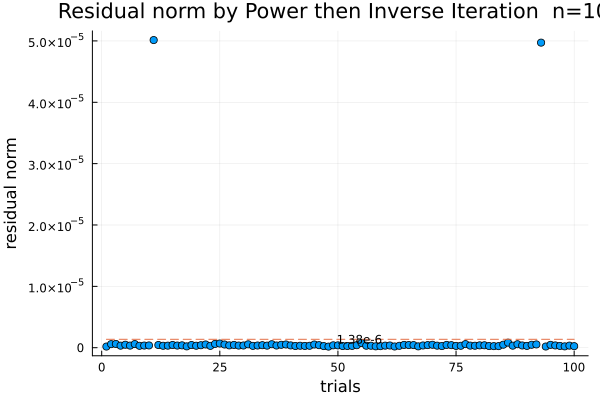
\includegraphics[width=72mm]{graphs/exp4_n100_residual.png} \\
    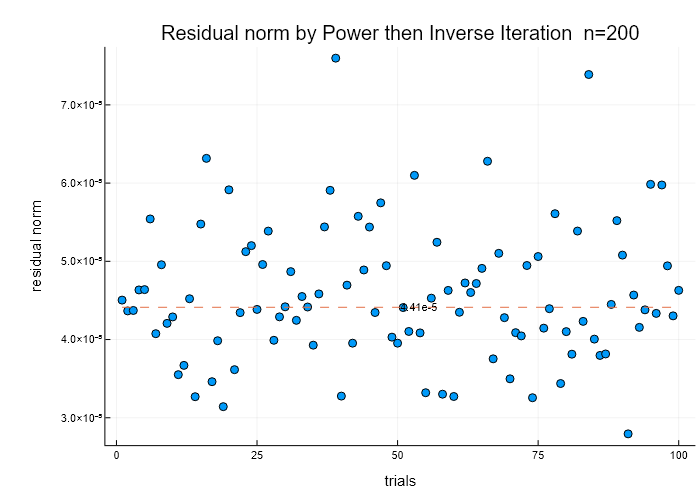
\includegraphics[width=72mm]{graphs/exp4_n200_residual.png} &
    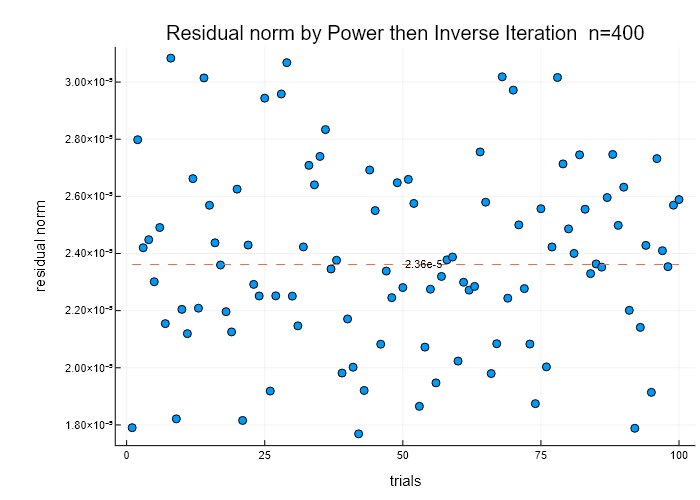
\includegraphics[width=72mm]{graphs/exp4_n400_residual.png} \\
  \end{tabular}
  \caption{逆反復法における固有方程式残差ノルム分布(各$N$)}
  \label{fig:exp4_residual}
\end{figure}

\begin{figure}[H]
  \centering
  \begin{tabular}{cc}
    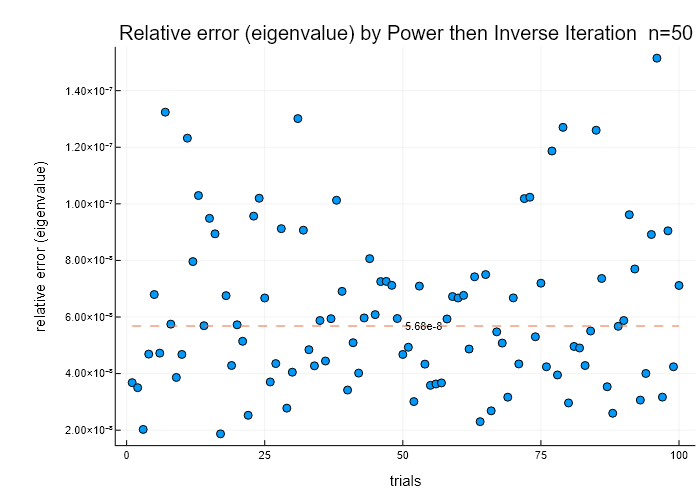
\includegraphics[width=72mm]{graphs/exp4_n50_relerr_eigenvalue.png} &
    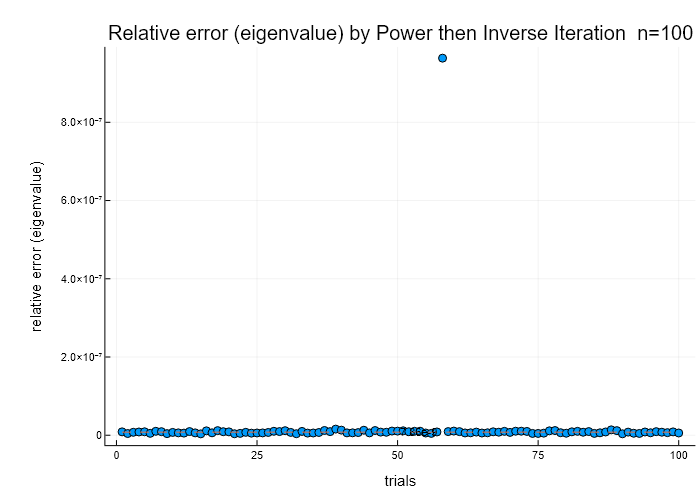
\includegraphics[width=72mm]{graphs/exp4_n100_relerr_eigenvalue.png} \\
    \includegraphics[width=72mm]{graphs/exp4_n200_relerr_eigenvalue.png} &
    \includegraphics[width=72mm]{graphs/exp4_n400_relerr_eigenvalue.png} \\
  \end{tabular}
  \caption{最大固有値の相対誤差分布(各$N$,逆反復法)}
  \label{fig:exp4_relerr_lambda}
\end{figure}

\begin{figure}[H]
  \centering
  \begin{tabular}{cc}
    \includegraphics[width=72mm]{graphs/exp4_n50_relerr_eigenvector.png} &
    \includegraphics[width=72mm]{graphs/exp4_n100_relerr_eigenvector.png} \\
    \includegraphics[width=72mm]{graphs/exp4_n200_relerr_eigenvector.png} &
    \includegraphics[width=72mm]{graphs/exp4_n400_relerr_eigenvector.png} \\
  \end{tabular}
  \caption{最大固有ベクトルの相対誤差分布(各$N$,逆反復法)}
  \label{fig:exp4_relerr_v}
\end{figure}

\begin{figure}[H]
  \centering
  \begin{tabular}{cc}
    \includegraphics[width=72mm]{graphs/exp4_n50_time.png} &
    \includegraphics[width=72mm]{graphs/exp4_n100_time.png} \\
    \includegraphics[width=72mm]{graphs/exp4_n200_time.png} &
    \includegraphics[width=72mm]{graphs/exp4_n400_time.png} \\
  \end{tabular}
  \caption{逆反復法の計算時間分布(各$N$)}
  \label{fig:exp4_time}
\end{figure}

\begin{figure}[H]
  \centering
  \begin{tabular}{cc}
    \includegraphics[width=72mm]{graphs/exp4_n50_iterations.png} &
    \includegraphics[width=72mm]{graphs/exp4_n100_iterations.png} \\
    \includegraphics[width=72mm]{graphs/exp4_n200_iterations.png} &
    \includegraphics[width=72mm]{graphs/exp4_n400_iterations.png} \\
  \end{tabular}
  \caption{逆反復法における収束までの反復回数分布(各$N$)}
  \label{fig:exp4_iterations}
\end{figure}

表\ref{tab:exp4_summary}に高速化の結果をまとめる。

\begin{table}[H]
\centering
\caption{逆反復法を用いた固有値計算の結果まとめ(100試行の中央値)}
\label{tab:exp4_summary}
\begin{tabular}{r|r|r|r|r|r}
\hline
$N$ & 残差ノルム & 固有値相対誤差 & 固有ベクトル相対誤差 & 計算時間 [s] & 反復回数 \\
\hline
50 & $1.396741\times10^{-6}$ & $5.550151\times10^{-8}$ & $4.561756\times10^{-16}$ & 0.000046 & 7.00 \\
100 & $3.569149\times10^{-7}$ & $7.120842\times10^{-9}$ & $4.624595\times10^{-16}$ & 0.000204 & 7.00 \\
200 & $4.561472\times10^{-5}$ & $4.549618\times10^{-7}$ & $5.279023\times10^{-16}$ & 0.001780 & 6.00 \\
400 & $2.302051\times10^{-5}$ & $1.150639\times10^{-7}$ & $6.452753\times10^{-16}$ & 0.010692 & 6.00 \\
\hline
\end{tabular}
\end{table}

\subsection{考察}
逆反復法を用いることで、収束までの反復回数は減少したものの、計算時間は増加した。これは、逆反復法が各反復で線形方程式を解く必要があり、そのためのLU分解が計算コストを押し上げたためである。\\

具体的には、LU分解に要する計算量は $O(N^3)$ であり全体の計算量は少なくとも$O(N^3)$ である、これに対しべき乗法の各反復は $O(N^2)$ で済むので反復回数を$k$とすると全体の計算量は、$O(N^2k)$ となる。今回の場合、べき乗法の反復回数$k$が10回程度のため、次元$n$が$k$に対して支配的であり、全体の計算時間がLU分解のコストに引きずられたと考えられる。\\

反復回数が極端に少ない理由として考えられるのは、実験方法で行列の生成を一様乱数であるrand()関数を用いているため、固有値同士の分離度が高く、収束が速まったためと考えられる。恣意的に固有値同士の分離度が低い行列を選択したり、正規分布の乱数randn()など他の分布を用いた場合、反復回数が増加し高速化が実現する可能性があるため、今後の課題として検討する価値がある。


\section{課題6:QR分解とQR法による固有値問題の解法}
\subsection{原理・方法}

QR分解(QR Decomposition)は,任意の正方行列 $A \in \mathbb{R}^{n\times n}$ をユニタリ行列 $Q$ と上三角行列 $R$ の積
\[
A = QR
\]
として表す手法である\cite{exp2025}.
ここで $Q^TQ = I$ が成り立つ.QR分解はグラム・シュミットの直交化に基づいて構成されるが,
数値的安定性を向上させるため,「修正グラム・シュミット法」が用いられる\cite{exp2025}.

修正版グラム・シュミット法では,行列 $A = (a_{1}, \ldots, a_{n})$ の各列ベクトル $a_{j}$ に対して次の手順を繰り返す:

\begin{align}
&\text{for } j = 1, \ldots, n \text{ do} \notag\\
&\quad R_{j,j} = \|a_{j}\|, \\
&\quad q_{j} = \frac{a_{j}}{R_{j,j}}, \\
&\quad \text{for } k = j+1, \ldots, n \text{ do} \notag\\
&\qquad R_{j,k} = q_{j}^{T} a_{k}, \\
&\qquad a_{k} \leftarrow a_{k} - R_{j,k} q_{j}, \\
&\quad \text{end for} \notag\\
&\text{end for} \notag
\end{align}

この手続きにより,$Q = (q_{1}, \ldots, q_{n})$ は直交行列,$R$ は上三角行列となり,
\[
A = QR
\]
が成り立つ。

本実験ではこの修正版アルゴリズムをJuliaで次のように実装した:

\begin{verbatim}
function qr_manual(A)
    n = size(A, 1)
    Q = copy(A)
    R = Matrix{eltype(A)}(I, n, n)
    for k = 1:n
        for j = 1:k-1
            R[j, k] = dot(Q[:, j], Q[:, k])
            Q[:, k] .-= R[j, k] * Q[:, j]
        end
        R[k, k] = norm(Q[:, k])
        Q[:, k] /= R[k, k]
    end
    return Q, R
end
\end{verbatim}

次に,QR法(QR Algorithm)は,このQR分解を反復的に適用して行列の固有値を求める手法である{\cite{exp2025}}.
初期行列 $A_{0} = A$ に対して以下の手順を繰り返す:
\begin{align}
A_{k} &= Q_{k} R_{k}, \\
A_{k+1} &= R_{k} Q_{k} (= Q_{k}^{-1} A_{k} Q_{k}).
\end{align}
これはユニタリ行列による相似変換の繰り返しであり,各 $A_{k}$ は $A$ と同じ固有値を持つ.
反復を続けると $A_{k}$ は上三角行列に近づき,その対角成分が固有値に収束する.
本実装では,収束判定条件
\[
\|A_{k+1} - A_k\|_{\infty} < \mathrm{tol} \cdot \|A_k\|_{\infty}
\]
を満たした時点で反復を停止し,対角成分を固有値として採用した.
また,求めた固有値を初期値として逆反復法を適用し,対応する固有ベクトルを得るようにした.

\begin{verbatim}
function qrEigens(A; max_iter=100000, tol=1e-10)
    n = size(A, 1)
    Ak = copy(A)
    eigenvectors = Matrix{Float64}(I, n, n)
    itr = 0
    for k in 1:max_iter
        itr += 1
        Q, R = qr_manual(Ak)
        Ak1 = R * Q
        if norm(Ak1 - Ak, Inf) < tol * norm(Ak, Inf)
            break
        end
        Ak = Ak1
    end
    eigenvalues = diag(Ak)
    for k in 1:n
        mu = eigenvalues[k]
        _, v_k = invEigen(A, mu, max_iter, tol)
        eigenvectors[:, k] = v_k
    end
    return eigenvalues, eigenvectors, itr
end
\end{verbatim}

QR法の理論的計算量は,各反復において $O(n^3)$(QR分解部分)を要するため,全体では $O(k n^3)$ である.
収束率はべき乗法と同様に一次であり,固有値の絶対値が近い場合は収束が遅くなる

\subsection{実験方法}

本課題では,QR分解を用いた固有値計算法(QR法)の性能を評価した.
対称行列 $A \in \mathbb{R}^{n \times n}$ を乱数により生成し,
QR法を適用して全固有値を求め,Julia の標準固有値関数 \texttt{eigen(A)} による真値と比較した.

次の関数 \verb|exp5| により,複数の行列サイズ $N$ に対して100回の試行を行い,
各試行における最大残差ノルム,固有値誤差,計算時間を記録した.

\begin{verbatim}
function exp5(N; num_trials=100)
    eigenvalues = zeros(num_trials, N)
    times       = zeros(num_trials)
    max_resnorms    = zeros(num_trials)
    max_relerrs_lambda = zeros(num_trials)
    itrs           = zeros(Int, num_trials)

    for t in 1:num_trials
        A = rand(N,N)
        A = (A + A') / 2             # 対称化
        λref = sort(eigen(A).values) # 参照値
        times[t] = @elapsed begin
            λ, V, itr = qrEigens(A)
        end
        eigenvalues[t, :] = λ
        itrs[t] = itr
        
        # 残差ノルム max_i ||(A - λ_i I)v_i||
        resnorms_i = zeros(N)
        for i in 1:N
            v_i = V[:, i]
            resnorms_i[i] = norm(A * v_i - λ[i] * v_i)
        end
        max_resnorms[t] = maximum(resnorms_i)
        
        # 相対誤差 max_i |λ_i - λ̂_i| / |λ_i|
        λ_sorted = sort(λ)
        relerrs_i = abs.(λ_sorted .- λref) ./ abs.(λref)
        max_relerrs_lambda[t] = maximum(relerrs_i)
    end

    (; max_resnorms, max_relerrs_lambda, times, itrs)
end
\end{verbatim}

ここで測定した量は次の通りである:
\begin{itemize}
  \item 最大残差ノルム $\displaystyle \max_i \| (A - \lambda_i I)\boldsymbol{v}_i \|$:固有対の再現精度を評価.
  \item 最大相対誤差 $\displaystyle \max_i \frac{|\lambda_i - \hat{\lambda}_i|}{|\lambda_i|}$:真値に対する固有値誤差.
  \item 計算時間:QR反復の収束までの所要時間.
\end{itemize}

各試行で得られた値の統計的変動を考慮するため,
中央値ではなく最大値を評価指標とし,
QR法の数値安定性と収束性能を比較できるよう設計した.


\subsection{結果(小問1)}
QR法による固有値計算の結果を図\ref{fig:exp5_residuals}~図\ref{fig:exp5_iterations}に示す.また,試行ごとの分布の概要を表\ref{tab:exp5_summary}に示す.行列サイズ $N=10, 20, 40, 80$ に対して10回の試行を行い,最大残差ノルム・最大固有値相対誤差・計算時間・反復回数を評価した.
また、本来は100回の試行を予定していたが、計算時間の都合上10回に変更した。
\begin{figure}[H]
  \centering
  \begin{tabular}{cc}
    \includegraphics[width=72mm]{graphs/exp5_n10_max_residual.png} &
    \includegraphics[width=72mm]{graphs/exp5_n20_max_residual.png} \\
    \includegraphics[width=72mm]{graphs/exp5_n40_max_residual.png} &
    \includegraphics[width=72mm]{graphs/exp5_n80_max_residual.png} \\
  \end{tabular}
  \caption{QR法における最大残差ノルム分布(各$N$)}
  \label{fig:exp5_residuals}
\end{figure}

\begin{figure}[H]
  \centering
  \begin{tabular}{cc}
    \includegraphics[width=72mm]{graphs/exp5_n10_max_relerr_eigenvalue.png} &
    \includegraphics[width=72mm]{graphs/exp5_n20_max_relerr_eigenvalue.png} \\
    \includegraphics[width=72mm]{graphs/exp5_n40_max_relerr_eigenvalue.png} &
    \includegraphics[width=72mm]{graphs/exp5_n80_max_relerr_eigenvalue.png} \\
  \end{tabular}
  \caption{QR法における最大固有値相対誤差分布(各$N$)}
  \label{fig:exp5_relerrs}
\end{figure}

\begin{figure}[H]
  \centering
  \begin{tabular}{cc}
    \includegraphics[width=72mm]{graphs/exp5_n10_time.png} &
    \includegraphics[width=72mm]{graphs/exp5_n20_time.png} \\
    \includegraphics[width=72mm]{graphs/exp5_n40_time.png} &
    \includegraphics[width=72mm]{graphs/exp5_n80_time.png} \\
  \end{tabular}
  \caption{QR法における計算時間分布(各$N$)}
  \label{fig:exp5_times}
\end{figure}

\begin{figure}[H]
  \centering
  \begin{tabular}{cc}
    \includegraphics[width=72mm]{graphs/exp5_n10_iterations.png} &
    \includegraphics[width=72mm]{graphs/exp5_n20_iterations.png} \\
    \includegraphics[width=72mm]{graphs/exp5_n40_iterations.png} &
    \includegraphics[width=72mm]{graphs/exp5_n80_iterations.png} \\
  \end{tabular}
  \caption{QR法における収束までの反復回数分布(各$N$)}
  \label{fig:exp5_iterations}
\end{figure}

\begin{table}[H]
\centering
\caption{QR法による固有値計算の結果まとめ(10試行の中央値)}
\label{tab:exp5_summary}
\begin{tabular}{r|r|r|r|r}
\hline
$N$ & 最大残差ノルム & 最大固有値相対誤差 & 計算時間 [s] & 反復回数 \\
\hline
10  & $2.31\times10^{-15}$ & $1.07\times10^{-14}$ & 0.343 & 283.5 \\
20  & $7.39\times10^{-15}$ & $3.66\times10^{-14}$ & 1.25 & 1128.0 \\
40  & $3.10\times10^{-13}$ & $2.57\times10^{-13}$ & 6.68 & 4551.0 \\
80  & $1.17\times10^{-10}$ & $8.29\times10^{-11}$ & 201.7 & 51532.0 \\
\hline
\end{tabular}
\end{table}

\subsection{考察(小問2,3)}
一番はN=80における反復回数が他のNの増加量に比べても病的に長い点である。最大残差ノルムが他よりも異様に大きいのも、反復回数が多く丸め誤差が蓄積したためだと考えられる。N=80における反復回数の増加は、相対誤差のとりうる最小の誤差が今回の設定した許容誤差よりも大きかったため、収束判定が厳しくなりすぎたことが原因と考えられ、実際N=40までの相対誤差の増加量を見ると少なくとも$O(N^2)$であり、N=80では$10^{-12}$を超えることが予想される。\\

N = 10, 20, 40における反復回数の増加量と計算時間はほぼ$O(N^2)$であり、$\frac{計算時間}{反復回数} $つまり、一回のループの計算時間がNの増加に対してほぼ一定であることが分かる。QR分解の計算量は$O(N^3)$であり、結果と矛盾するように見えるが、今回の実験範囲ではNのサンプルが少なく、また試行回数も10回と少ないため、計算量の理論値が反映されなかったと考えられる。\\

\section{課題7:QR法}
\subsection{原理・方法}

QR法の高速化には,「シフト(shift)」と「減次(deflation)」の2つの戦略が用いられる\cite{exp2025}.

\paragraph{シフトによる収束の加速}
行列 $A$ に対して定数 $\sigma$ を引いた
\[
A' = A - \sigma I
\]
という変換を行う操作をシフトという{\cite{exp2025}}.
$A$ の固有値が $\lambda_{1}, \ldots, \lambda_{n}$ のとき,
シフト後の行列 $A'$ の固有値は $\lambda_{i} - \sigma$ である.

QR法の反復中で,例えば第 $n$ 固有値 $\lambda_{n}$ の近似値 $\sigma$ が得られたとき,
次の反復を $A_{k} - \sigma I$ に対して行うことで収束を加速できる.
特に $\sigma$ が $\lambda_{n}$ に近ければ,
行列 $A_{k}$ の下三角成分の収束率
\[
\rho'_{i,j} = \frac{|\lambda_{i} - \sigma|}{|\lambda_{j} - \sigma|}
\]
はシフト前の収束率 $\rho_{i,j} = |\lambda_{i}| / |\lambda_{j}|$ より小さくなり,
第 $n$ 行要素の収束が著しく速くなる.

\paragraph{減次による計算量削減}
QR法を繰り返すと,行列 $A_{k}$ の第 $n$ 行成分がほぼゼロになる(すなわち下三角要素が十分に小さい)時点が現れる.
すなわち,ある閾値 $\varepsilon$ に対して
\[
\frac{|a_{k;n,j}|}{|a_{k;n,n}|} < \varepsilon \quad (1 \le j < n)
\]
が成立すれば,$A_{k}$ は
\[
A_{k} \approx
\begin{pmatrix}
B_{k} & * \\
0 & a_{k;n,n}
\end{pmatrix}
\]
の形となる.ここで $B_{k}$ は $A_{k}$ の左上 $(n-1)\times(n-1)$ の部分行列であり,
固有値は $a_{k;n,n}$ と $B_{k}$ の固有値で近似できる.
このとき $a_{k;n,n}$ を1つの固有値として確定させ,
以後の反復を $B_{k}$ に対してのみ続けることで,
行列のサイズを1つ減らし計算量を削減できる{\cite{exp2025}}.
この手続きを「減次」と呼ぶ.


本課題では,これらの戦略を組み合わせた高速QR法をJuliaで実装した.
以下にその主要部を示す:

\begin{verbatim}
function qrEigens_fast(A; max_iter=100000, tol=1e-10)
    n = size(A, 1)
    Ak = copy(A)
    itr = 0
    mu = 0.0
    dimension = n
    eigenvalues = zeros(n)
    eigenvectors = Matrix{Float64}(I, n, n)

    for k in 1:max_iter
        itr += 1
        L = Matrix{eltype(Ak)}(I, dimension, dimension)
        # --- 減次判定 ---
        if norm((Ak - mu*L)[dimension, 1:dimension-1], 1) < tol
            eigenvalues[dimension] = Ak[dimension, dimension]
            dimension -= 1
            Ak = Ak[1:dimension, 1:dimension]
            if dimension == 0
                break
            end
        end
        # --- シフト付きQR反復 ---
        mu = Ak[dimension, dimension]
        Q, R = qr_manual(Ak - mu*L)
        Ak1 = R * Q + mu * L
        if norm(Ak1 - Ak, Inf) < tol * norm(Ak, Inf)
            eigenvalues[1:dimension] = diag(Ak1)
            break
        end
        Ak = Ak1
    end
    # --- 固有ベクトルは逆反復法で算出 ---
    for k in 1:n
        mu = eigenvalues[k]
        _, v_k = invEigen(A, mu, 1000, tol)
        eigenvectors[:, k] = v_k
    end
    return eigenvalues, eigenvectors, itr
end
\end{verbatim}

この方法により,従来のQR法に比べて収束速度が向上し,
計算量を効果的に削減することができる.

\subsection{実験方法}
課題6と同一の評価系を用いる.対称行列 $A\in\mathbb{R}^{N\times N}$ を乱数から生成・対称化し,高速化QR法(シフト+減次)\verb|qrEigens_fast| を適用する.各 $N$ について10回試行し,(i) 最大残差ノルム $\max_{i}\|(A-\lambda_{i} I)\boldsymbol{v}_{i}\|$,(ii) 固有値の最大相対誤差 $\max_{i} |\lambda_{i}-\hat{\lambda}_{i}|/|\lambda_{i}|$(参照は \verb|eigen(A)|),(iii) 計算時間,(iv) 反復回数を記録し,代表値として中央値を用いる.

\begin{verbatim}
function exp6(N; num_trials=100)
    eigenvalues = zeros(num_trials, N)
    times       = zeros(num_trials)
    max_resnorms    = zeros(num_trials)
    max_relerrs_lambda = zeros(num_trials)
    itrs           = zeros(Int, num_trials)

    for t in 1:num_trials
        A = rand(N,N)
        A = (A + A') / 2            # 対称化
        λref = sort(eigen(A).values)
        times[t] = @elapsed begin
            λ, V, itr = qrEigens_fast(A)
        end
        eigenvalues[t, :] = λ
        itrs[t] = itr
        # 残差ノルム(最大)
        resnorms_i = zeros(N)
        for i in 1:N
            v_i = V[:, i]
            resnorms_i[i] = norm(A * v_i - λ[i] * v_i)
        end
        max_resnorms[t] = maximum(resnorms_i)
        # 固有値の最大相対誤差
        λ_sorted = sort(λ)
        relerrs_i = abs.(λ_sorted .- λref) ./ abs.(λref)
        max_relerrs_lambda[t] = maximum(relerrs_i)
    end
    (; max_resnorms, max_relerrs_lambda, times, itrs)
end
\end{verbatim}

違いはアルゴリズム本体のみ(シフトと減次を併用)であり,評価指標・統計処理は課題6と同じである.


\subsection{結果}
高速化QR法(シフト+減次)による固有値計算の結果を図\ref{fig:exp6_residuals}~図\ref{fig:exp6_iterations}に示す.また,試行ごとの分布の概要を表\ref{tab:exp6_summary}に示す.行列サイズ $N=10, 20, 40, 80$ に対して10回の試行を行い,最大残差ノルム・最大固有値相対誤差・計算時間・反復回数を評価した.

\begin{figure}[H]
  \centering
  \begin{tabular}{cc}
    \includegraphics[width=72mm]{graphs/exp6_n10_max_residual.png} &
    \includegraphics[width=72mm]{graphs/exp6_n20_max_residual.png} \\
    \includegraphics[width=72mm]{graphs/exp6_n40_max_residual.png} &
    \includegraphics[width=72mm]{graphs/exp6_n80_max_residual.png} \\
  \end{tabular}
  \caption{高速化QR法における最大残差ノルム分布(各$N$)}
  \label{fig:exp6_residuals}
\end{figure}

\begin{figure}[H]
  \centering
  \begin{tabular}{cc}
    \includegraphics[width=72mm]{graphs/exp6_n10_max_relerr_eigenvalue.png} &
    \includegraphics[width=72mm]{graphs/exp6_n20_max_relerr_eigenvalue.png} \\
    \includegraphics[width=72mm]{graphs/exp6_n40_max_relerr_eigenvalue.png} &
    \includegraphics[width=72mm]{graphs/exp6_n80_max_relerr_eigenvalue.png} \\
  \end{tabular}
  \caption{高速化QR法における最大固有値相対誤差分布(各$N$)}
  \label{fig:exp6_relerrs}
\end{figure}

\begin{figure}[H]
  \centering
  \begin{tabular}{cc}
    \includegraphics[width=72mm]{graphs/exp6_n10_time.png} &
    \includegraphics[width=72mm]{graphs/exp6_n20_time.png} \\
    \includegraphics[width=72mm]{graphs/exp6_n40_time.png} &
    \includegraphics[width=72mm]{graphs/exp6_n80_time.png} \\
  \end{tabular}
  \caption{高速化QR法における計算時間分布(各$N$)}
  \label{fig:exp6_times}
\end{figure}

\begin{figure}[H]
  \centering
  \begin{tabular}{cc}
    \includegraphics[width=72mm]{graphs/exp6_n10_iterations.png} &
    \includegraphics[width=72mm]{graphs/exp6_n20_iterations.png} \\
    \includegraphics[width=72mm]{graphs/exp6_n40_iterations.png} &
    \includegraphics[width=72mm]{graphs/exp6_n80_iterations.png} \\
  \end{tabular}
  \caption{高速化QR法における収束までの反復回数分布(各$N$)}
  \label{fig:exp6_iterations}
\end{figure}

\begin{table}[H]
\centering
\caption{高速化QR法による固有値計算の結果まとめ(10試行の中央値)}
\label{tab:exp6_summary}
\begin{tabular}{r|r|r|r|r}
\hline
$N$ & 最大残差ノルム & 最大固有値相対誤差 & 計算時間 [s] & 反復回数 \\
\hline
10  & $2.08\times10^{-15}$ & $9.94\times10^{-15}$ & 0.00297 & 22.0 \\
20  & $2.86\times10^{-15}$ & $2.50\times10^{-14}$ & 0.0166 & 44.5 \\
40  & $1.17\times10^{-14}$ & $1.68\times10^{-14}$ & 0.0649 & 85.5 \\
80  & $4.10\times10^{-14}$ & $5.63\times10^{-14}$ & 0.392 & 179.0 \\
\hline
\end{tabular}
\end{table}

\subsection{考察}
課題6と比べて、反復回数、計算時間ともに大幅に削減されており、それに伴い丸め誤差による最大残差ノルム、最大固有値相対誤差も軽減されたことが確認できた。特にN=80における反復回数の増加量が他のNに比べても抑えられており、シフトと減次の効果が顕著であることが示されている。\\

反復回数が$O(N)$であるのは、シフトにより高々定数回の反復で一つの固有値が確定し、行列の次元が1ずつ減少していくためである。
\section{結論}

本章では,数値線形代数における主要なアルゴリズムを実装・評価した.各課題において実装したアルゴリズムの数値的特性は,線形代数の理論と基本的に一致していることが確認できた.一方,ランダムに生成された行列データを用いることで,全課題を通して外れ値やランダム要素が顕著に現れたことが観測された。つまり、行列の条件数がランダムに変動するため,各試行ごとに計算精度や収束速度にばらつきが生じ、 特に条件の悪いケースが稀に現れることで,最大誤差や計算時間の分布に長い裾が生じた.課題6では試行回数が少なく、このようなランダム要素に影響されたため、計算量が理論通りに行かなかったと考えられる。これらの現象は,理論的には平均的な挙動をよく説明する一方で,実装レベルでは統計的なばらつきを含む実践的な理解が重要であることを示唆している.\\

結論として,本実験は数値線形代数の理論と計算機実装の関係を具体的に学ぶ良い教材となった.同時に,ランダム行列に由来する外れ値やばらつきの影響を理解することが,実際の数値計算において重要であることを示した.今後の課題として,より堅牢なアルゴリズム設計や,ランダム性を考慮した数値解析手法の開発が期待される.
\section*{付録(Appendix)}
\begin{itemize}
  \item 使用したソースコード(Julia/Python)
  \url{https://github.com/Issan0511/suuri_exp/blob/master/1/julia1.ipynb}
  \item AI補完の使用: Juliaコードの一部およびレポートの一部において、GPT-5およびClaude Sonnet 4.5の補完を使用した。
\end{itemize}

\section*{参考文献(References)}
\begin{thebibliography}{99}
\bibitem{exp2025} 数理工学実験(2025年度配布資料).
\end{thebibliography}


\end{document}
